\documentclass[12pt]{article}
\usepackage[margin=2.5cm]{geometry}
\usepackage{enumerate}
\usepackage{amsfonts}
\usepackage{amsmath}
\usepackage{fancyhdr}
\usepackage{amsmath}
\usepackage{amssymb}
\usepackage{amsthm}
\usepackage{mdframed}
\usepackage{graphicx}
\usepackage{subcaption}
\usepackage{adjustbox}
\usepackage{listings}
\usepackage{xcolor}
\usepackage{courier}
\usepackage[utf]{kotex}
\usepackage{hyperref}
\usepackage{soul}

\definecolor{codegreen}{rgb}{0,0.6,0}
\definecolor{codegray}{rgb}{0.5,0.5,0.5}
\definecolor{codepurple}{rgb}{0.58,0,0.82}
\definecolor{backcolour}{rgb}{0.95,0.95,0.92}

\lstdefinestyle{mystyle}{
    backgroundcolor=\color{backcolour},
    commentstyle=\color{codegreen},
    keywordstyle=\color{magenta},
    numberstyle=\tiny\color{codegray},
    stringstyle=\color{codepurple},
    basicstyle=\ttfamily\footnotesize,
    breakatwhitespace=false,
    breaklines=true,
    captionpos=b,
    keepspaces=true,
    numbers=left,
    numbersep=5pt,
    showspaces=false,
    showstringspaces=false,
    showtabs=false,
    tabsize=1
}

\lstset{style=mystyle}

\pagestyle{fancy}
\renewcommand{\headrulewidth}{0.4pt}
\lhead{CSC 369}
\rhead{Midterm 4 Solution}

\begin{document}
\title{CSC 369 Midterm 4 Solution}

\bigskip

\begin{enumerate}[1.]
    \item

    \begin{enumerate}[a)]

        \item
        \begin{enumerate}[1)]
            \item 4 - inode blocks. 1 for the file \texttt{c}, and 3 for the
            directdories \texttt{/}, \texttt{a}, \texttt{b}

            \item 3 - directory blocks - one for root \texttt{/}, one for \texttt{a},
            the other for \texttt{b}

            \item 1 - single indirect block as far as we know. The file definitely has more than
            12 blocks (\# of data blocks pointed by direct pounters), but less than 1036 (\# of data blocks pointed
            by direct pointers and single indirect pointers). We are reading block 1034.

            \item 1 - data block for file \texttt{c}
        \end{enumerate}
    \end{enumerate}

    \item

    \begin{enumerate}
        \item

        All of the above

        \bigskip

        \underline{\textbf{Notes}}

        \begin{itemize}
            \item \textbf{Inode}

            \begin{center}
            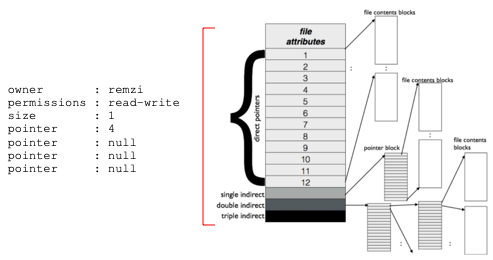
\includegraphics[width=0.8\linewidth]{../images/midterm_4_solution_1.png}
            \end{center}

            \begin{itemize}
                \item Is short form of \textbf{index node}
                \item Describes a file system object such as file or data
                \item Contains all information about a file/directory, including
                \begin{itemize}
                    \item File Type,
                    \item Size
                    \item Number of blocks allocated to it
                    \item Protection information
                    \item Time information (e.g time created, time modified)
                    \item Location of data blocks residing on disk
                \end{itemize}

            \end{itemize}
        \end{itemize}

        \bigskip

        \underline{\textbf{References}}

        \begin{enumerate}[1)]
            \item Wikipedia, Inode, \href{https://en.wikipedia.org/wiki/Inode}{link}
            \item Machanick, Philip. (2016). Teaching Operating Systems: Just Enough Abstraction. 642. 10.1007/978-3-319-47680-3\_10., \href{https://www.researchgate.net/figure/Conceptual-index-node-inode-The-top-level-block-contains-file-attributes-12-direct_fig1_306347325}{link}
        \end{enumerate}

        \item

        Size, the location of data blocks that reside on disk

        \bigskip

        \underline{\textbf{Notes}}

        \begin{itemize}
            \item I wonder what information about blocks inode has. Is it total number
            of blocks both inode and data, or just data?
            \item I struggled a bit on this one. I should find an easier way to
            remember which information inode has
        \end{itemize}

        \item

        \begin{itemize}
            \item \textbf{Inode Bitmap and Data Block Bitmap}

            \bigskip

            \texttt{(b) - Data Leak}

            \texttt{(c) - Inode Leak}

            \item \textbf{New Directory Inode}

            \bigskip

            \texttt{(a) - No inconsistency}

            \item \textbf{Inode Bitmap}, \textbf{Data Block Bitmap}, \textbf{Existing Directory Data},
            \textbf{New Directory Inode}, and \textbf{New Directory Data}

            \bigskip

            \texttt{(e) - Inconsistent inode data}

            \item \textbf{Inode Bitmap}, and \textbf{New Directory Inode}

            \bigskip

            \texttt{(c) - Inode leak}

            \texttt{(d) - Multiple file paths may point to same inode}

            \item \textbf{New Directory Inode}, \textbf{Existing Directory Inode}, \textbf{Existing Directory Data}

            \bigskip

            \texttt{(e) - Inconsistent inode data}

            \texttt{(f) - Something points to garbage}
        \end{itemize}

        \bigskip

        \begin{mdframed}
        \underline{\textbf{Correct Solution}}

        \bigskip

        \begin{itemize}
            \item \textbf{Inode Bitmap and Data Block Bitmap}

            \bigskip

            \texttt{(b) - Data Leak}

            \texttt{(c) - Inode Leak}

            \item \textbf{New Directory Inode}

            \bigskip

            \texttt{(a) - No inconsistency}

            \item \textbf{Inode Bitmap}, \textbf{Data Block Bitmap}, \textbf{Existing Directory Data},
            \textbf{New Directory Inode}, and \textbf{New Directory Data}

            \bigskip

            \texttt{(e) - Inconsistent inode data}

            \item \textbf{Inode Bitmap}, and \textbf{New Directory Inode}

            \bigskip

            \texttt{(c) - Inode leak}

            \item \textbf{New Directory Inode}, \textbf{Existing Directory Inode}, \textbf{Existing Directory Data}

            \bigskip

            \color{red}\texttt{(d) - Multiple file paths may point to same inode}\color{black}

            \texttt{(f) - Something points to garbage}
        \end{itemize}


        \end{mdframed}

        \bigskip

        % \underline{\textbf{Rough Work}}

        % \begin{itemize}
        %     \item \textbf{Creash Scenarios}

        %     \begin{itemize}
        %         \item When only new data block is written to disk

        %         \begin{itemize}
        %             \item This is fine in system's point of view
        %             \item No inode points to it (it doesn't contain any information about file)
        %             \item No bitmap points to it
        %             \item Is as if write never occured
        %         \end{itemize}
        %         \item When only the updated inode is written to disk
        %         \begin{itemize}
        %             \item There is no bitmap that's pointing to it
        %             \item There is new inode where existing inode is
        %             \item The data block \texttt{Db} hasn't been created
        %             \item Reading data where \texttt{Db} is will return garbage data
        %             \item there is a term for this. Is called \textbf{File-System inconsistency}
        %         \end{itemize}
        %         \item When only inode bitmap is written to disk

        %         \begin{itemize}
        %             \item inode block pointed by bitmap is assumed to be allocated
        %             \item But there is no desired inode where it's pointing
        %             \item This is another example of \textbf{File-System-Inconsistency}
        %             \item If left as is, then space cannot be used for future use (\textbf{inode leak})
        %         \end{itemize}
        %         \item When only data bitmap is written to disk

        %         \begin{itemize}
        %             \item data block pointed by bitmap is assumed to be allocated
        %             \item But there is no desired inode where it's pointing
        %             \item This is another example of \textbf{File-System-Inconsistency}
        %             \item If left as is, then space cannot be used for future use (\textbf{data leak})
        %         \end{itemize}
        %     \end{itemize}
        % \end{itemize}

        \bigskip

        \underline{\textbf{Notes}}

        \begin{itemize}
            \item I wonder how system call for reading file/directory works in UNIX. Does it check for bitmap?
            \item I wonder how system call for deleting file/directory works in UNIX
            \item I wonder how system call for creatubg file/directory works in UNIX
            \item Learned that
            \begin{itemize}
                \item Missing Inode Bitmap - multiple file paths may point to same inode
            \end{itemize}
            \item \textbf{File API}
            \begin{itemize}
                \item \texttt{open} (create/access file)
                \begin{itemize}
                    \item Is a system call
                    \item Reads target inode into memory (when loading)
                    \item Does three things on creation

                    \begin{enumerate}[1)]
                        \item make structure (inode) that racks all relevant information about file
                        \item link human readible name to the file, and put that link to a directory
                        \item increment \textbf{reference count} in inode
                    \end{enumerate}

                    \item \textbf{Syntax:}

                    \bigskip

                    \texttt{int fd = open("foo". O\_CREAT|O\_WRONLY|O\_TRUNC, S\_IRUSR|S\_IWUSR)}

                    \bigskip

                    \begin{itemize}
                        \item \texttt{O\_CREAT} - Creates file "foo" if does not exist
                        \item \texttt{O\_WRONLY} - Open file for writing only (default)
                        \item \texttt{O\_TRUNC} - Overwrites existing file \color{red}Need example/Clarification\color{black}
                        \item Can have multiple flags
                    \end{itemize}
                    \item Returns \textbf{file descriptor} or \texttt{fd} for short

                    \begin{itemize}
                        \item Is an integer
                        \item Is used to access a file
                        \item Is \underline{private} per process
                        \item Can be used to \texttt{read()} and \texttt{write()} files
                    \end{itemize}

                    \bigskip

                    \underline{\textbf{Example}}

                    \bigskip

                    \begin{center}
                    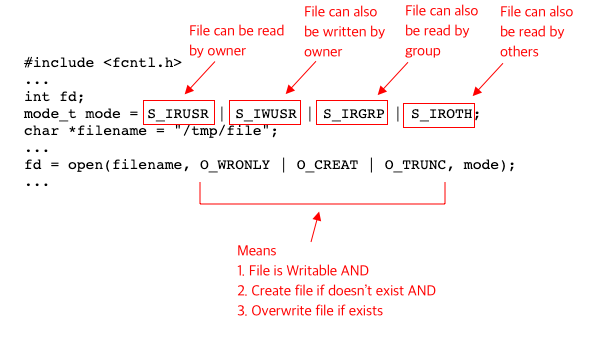
\includegraphics[width=\linewidth]{../images/midterm_4_solution_2.png}
                    \end{center}

                    \item Amount of I/O generated by \texttt{open()} is proportional to length
                    of pathname (wait. How is I/O involved in open()?)

                    \bigskip

                \end{itemize}

                \item \texttt(read) (read file)
                \begin{itemize}
                    \item Is a system call
                    \item \textbf{Syntax:}

                    \bigskip

                    \texttt{ssize\_t read (int fd, void *buf, size\_t count)}

                    \bigskip

                    \begin{itemize}
                        \item \texttt{fd} - file descriptor (from \texttt{open()})
                        \item \texttt{buf} - container for the read data
                        \item \texttt{count} - number of bytes to read
                    \end{itemize}
                    \item Returns number of bytes read, if successful
                    \item Returns 0 if is at, or past the end of file

                    \bigskip

                    \underline{\textbf{Example}}

                    \bigskip

                    \begin{center}
                    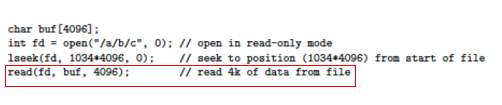
\includegraphics[width=\linewidth]{../images/midterm_4_solution_3.png}
                    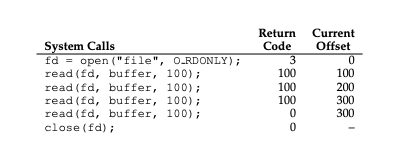
\includegraphics[width=\linewidth]{../images/midterm_4_solution_5.png}
                    \end{center}

                \end{itemize}

                \item \texttt{write} (write file)

                \begin{itemize}
                    \item Is a system call
                    \item Writes data out of a buffer
                    \item \textbf{Syntax:}

                    \bigskip

                    \texttt{ssize\_t write (int fd, const void * buf, size\_t nbytes)}

                    \bigskip

                    \begin{itemize}
                        \item \texttt{fd} - file descriptor
                        \item \texttt{buf} - A pointer to a buffer to write to file
                        \item \texttt{nbytes} - number of bytes to write. If smaller than buffer, the output is truncated
                    \end{itemize}
                \end{itemize}

                \bigskip

                \underline{\textbf{Example}}

                \bigskip

                \begin{center}
                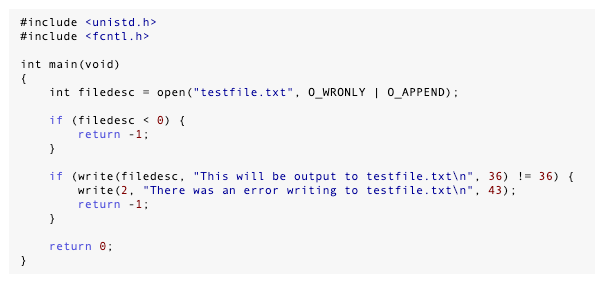
\includegraphics[width=\linewidth]{../images/midterm_4_solution_4.png}
                \end{center}

                \item \texttt{lseek}

                \begin{itemize}
                    \item Reads or write to a specific offset within a file
                    \item \textbf{Syntax:}

                    \bigskip

                    \texttt{off\_t lseek (int fd, off\_t offset, int whence)}

                    \bigskip

                    \begin{itemize}
                        \item \texttt{fd} - file descriptor
                        \item \texttt{offset} - the offset of pointer within file (in bytes)
                        \item \texttt{whence} - the method of offset

                        \bigskip

                        \quad \texttt{SEEK\_SET}  - offset from the start of file (absolute)

                        \quad \texttt{SEEK\_CUR} - offset from current location + offset bytes (relative)

                        \quad \texttt{SEEK\_END} - offset from the end of file
                    \end{itemize}

                    \item Returns offset amount (in bytes) from the \underline{beginning} of file
                    \item Returns -1 if error
                \end{itemize}

                \bigskip

                \underline{\textbf{Example}}

                \begin{center}
                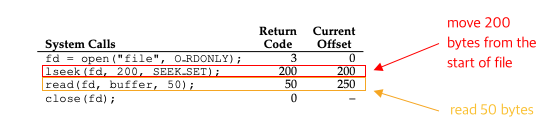
\includegraphics[width=\linewidth]{../images/midterm_4_solution_7.png}
                \end{center}

                \item \texttt{rename} (update file name)

                \begin{itemize}
                    \item Is a system call
                    \item Changes the name of file
                    \item Is \textbf{atomic} (after crash, it will be either old or new, but not in-between)
                    \item \textbf{Syntax:} \texttt{int rename(const char *old, const char *new)}

                    \begin{itemize}
                        \item \texttt{old} - name of old file
                        \item \texttt{new} - name of new file
                    \end{itemize}

                    \item Returns 0 if successful
                    \item Returns -1 if error
                \end{itemize}

                \bigskip

                \underline{\textbf{Example}}

                \begin{center}
                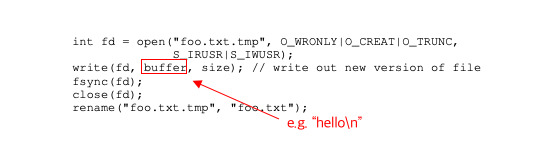
\includegraphics[width=\linewidth]{../images/midterm_4_solution_8.png}
                \end{center}

                \item \texttt{stat} (get file info)

                \begin{itemize}
                    \item displays metadata of a certain file stored in \textbf{inode}
                    \item \textbf{Syntax:} \texttt{int stat(const char *path, struct stat *buf)}

                    \begin{itemize}
                        \item \texttt{path} - file descriptor of file that's being inquired
                        \item \texttt{buf} - A \texttt{stat} structure where data about the file will be stored (see below)

                        \bigskip

                        \begin{center}
                        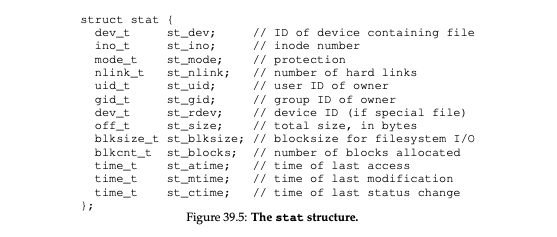
\includegraphics[width=\linewidth]{../images/midterm_4_solution_9.png}
                        \end{center}
                    \end{itemize}
                \end{itemize}

                \bigskip

                \underline{\textbf{Example}}

                \begin{center}
                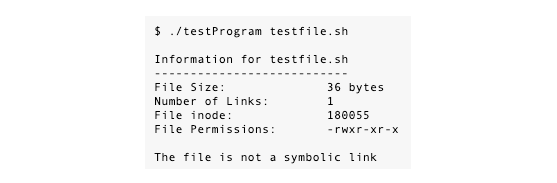
\includegraphics[width=\linewidth]{../images/midterm_4_solution_10.png}
                \end{center}

                \bigskip

                The result of above is:

                \begin{center}
                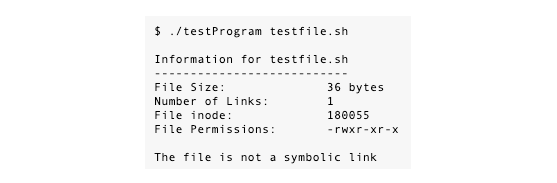
\includegraphics[width=\linewidth]{../images/midterm_4_solution_11.png}
                \end{center}
            \end{itemize}

            \item \texttt{unlink} (removing file)

            \begin{itemize}
                \item Is a system call
                \item Removes a \underline{file} (including symbolic link) from the system
                \item \textbf{Syntax:} \texttt{int unlink(const char *pathname)}

                \begin{itemize}
                    \item \texttt{pathname} - path to file
                \end{itemize}

                \item Returns 0 if successful
                \item Returns -1 if error
            \end{itemize}

            \bigskip

            \underline{\textbf{Example}}

            \begin{center}
            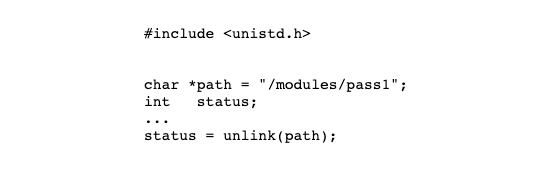
\includegraphics[width=\linewidth]{../images/midterm_4_solution_12.png}
            \end{center}

            \item \texttt{mkdir} (creating directory)

            \begin{itemize}
                \item Is a system call
                \item \textbf{Syntax:} \texttt{int mkdir(const char *path, mode\_t mode)}
                \begin{itemize}
                    \item \texttt{path} - path of directory (including name)
                    \item \texttt{mode} - permission group
                \end{itemize}
                \item Returns 0 if successful
                \item Returns -1 if error
                \item directories can never be written directly
                \begin{itemize}
                    \item directory is in format called \textbf{File System Metadata}
                    \item directory can \underline{only} be updated directly
                \end{itemize}
                \item creates two directories on creation \texttt{.} (current) and \texttt{..} (parent)
            \end{itemize}

            \bigskip

            \underline{\textbf{Example}}

            \begin{center}
            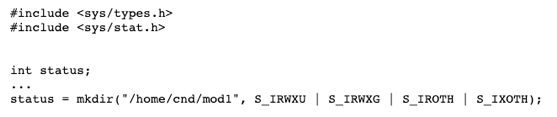
\includegraphics[width=\linewidth]{../images/midterm_4_solution_13.png}
            \end{center}

            \item \texttt{opendir, readdir, closedir} (reading directory)

            \begin{itemize}
                \item Are system calls
                \item Are under \texttt{$<$dirent.h$>$} library
                \item Requires \texttt{struct dirent} data structure

                \begin{center}
                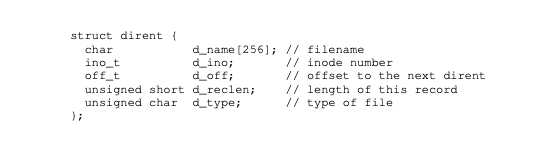
\includegraphics[width=\linewidth]{../images/midterm_4_solution_14.png}
                \end{center}

                \item \textbf{Syntax (opendir): } \texttt{DIR *opendir(const char *dirname)}
                \begin{itemize}
                    \item \texttt{dirname} - directory path
                    \item Returns a pointer to the directory stream
                    \item The stream is positioned at \underline{the first entry} in the directory.
                \end{itemize}
                \item \textbf{Syntax (readdir): } \texttt{struct dirent *readdir(DIR *dirp);}
                \begin{itemize}
                    \item \texttt{dirp} - directory stream
                    \item Returns a pointer to a dirent structure representing the next directory entry in the directory stream
                    \item Returns NULL on reaching the end of the directory stream
                \end{itemize}
                \item \textbf{Syntax (closedir): } \texttt{int closedir(DIR *dirp));}
                \begin{itemize}
                    \item \texttt{dirp} - directory stream
                    \item Returns 0 if successful
                    \item Returns -1 otherwise
                \end{itemize}

                \bigskip

                \underline{\textbf{Example}}

                \bigskip

                \begin{center}
                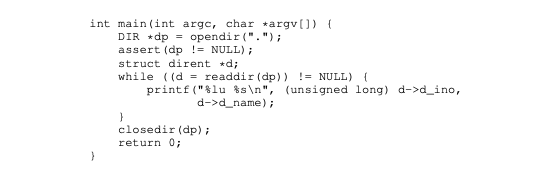
\includegraphics[width=\linewidth]{../images/midterm_4_solution_15.png}
                \end{center}

            \end{itemize}

            \item \text{rmdir} (Deleting Directories)

            \begin{itemize}
                \item Removes a directory whose name is given by path
                \item Is performed only when directory is empty
                \item Is included in \texttt{$<$unistd.h$>$} library
                \item Fails if is symbolic link
                \item \textbf{Syntax:} \texttt{int rmdir(const char *path)}

                \begin{itemize}
                    \item \texttt{path} - path of directory
                \end{itemize}
                \item Returns 0 if successful
                \item Returns -1 if error
            \end{itemize}

            \bigskip

            \underline{\textbf{Example}}

            \begin{center}
            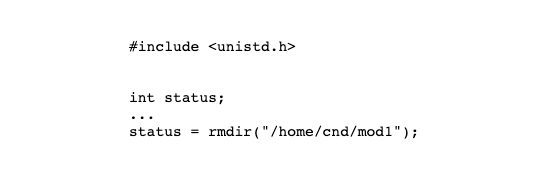
\includegraphics[width=\linewidth]{../images/midterm_4_solution_16.png}
            \end{center}

            \item \texttt{unlink} (Remove file)

            \begin{itemize}
                \item Remove a link to a file
                \item Is called \textbf{unlink} because it decrements \textbf{reference count} in inode
                \begin{itemize}
                    \item Deletes file completely when reference count within the inode number is 0
                \end{itemize}
                \item \textbf{Syntax:}

                \bigskip
                \texttt{\#include $<$unistd.h$>$}

                \bigskip

                \texttt{int unlink(const char *pathname);}

                \bigskip

                \begin{itemize}
                    \item \texttt{pathname} - pathname to file
                \end{itemize}
                \item Returns 0 if successful
                \item Returns -1 if error
                \item Is used by linux command \texttt{rm}
            \end{itemize}

            \bigskip

            \underline{\textbf{Example}}

            \begin{center}
            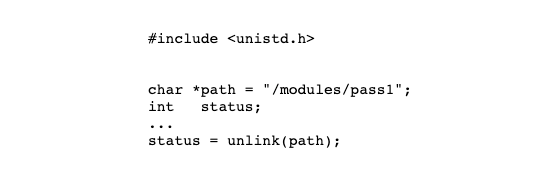
\includegraphics[width=\linewidth]{../images/midterm_4_solution_17.png}
            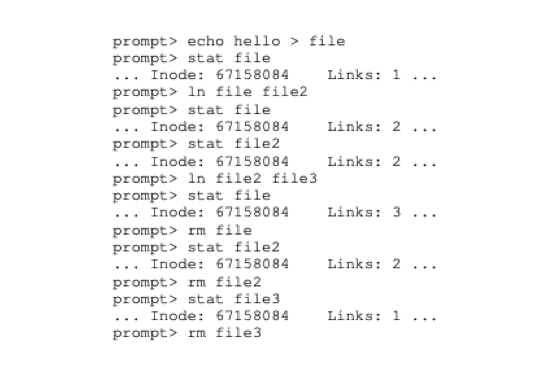
\includegraphics[width=\linewidth]{../images/midterm_4_solution_18.png}
            \end{center}

            \item \textbf{Symbolic Link:}
            \begin{itemize}
                \item Is directory entry containing "true" path to the file
                \item Is a shortcut that reference to a file instead of inode value $^{[2]}$
            \end{itemize}

            \begin{center}
                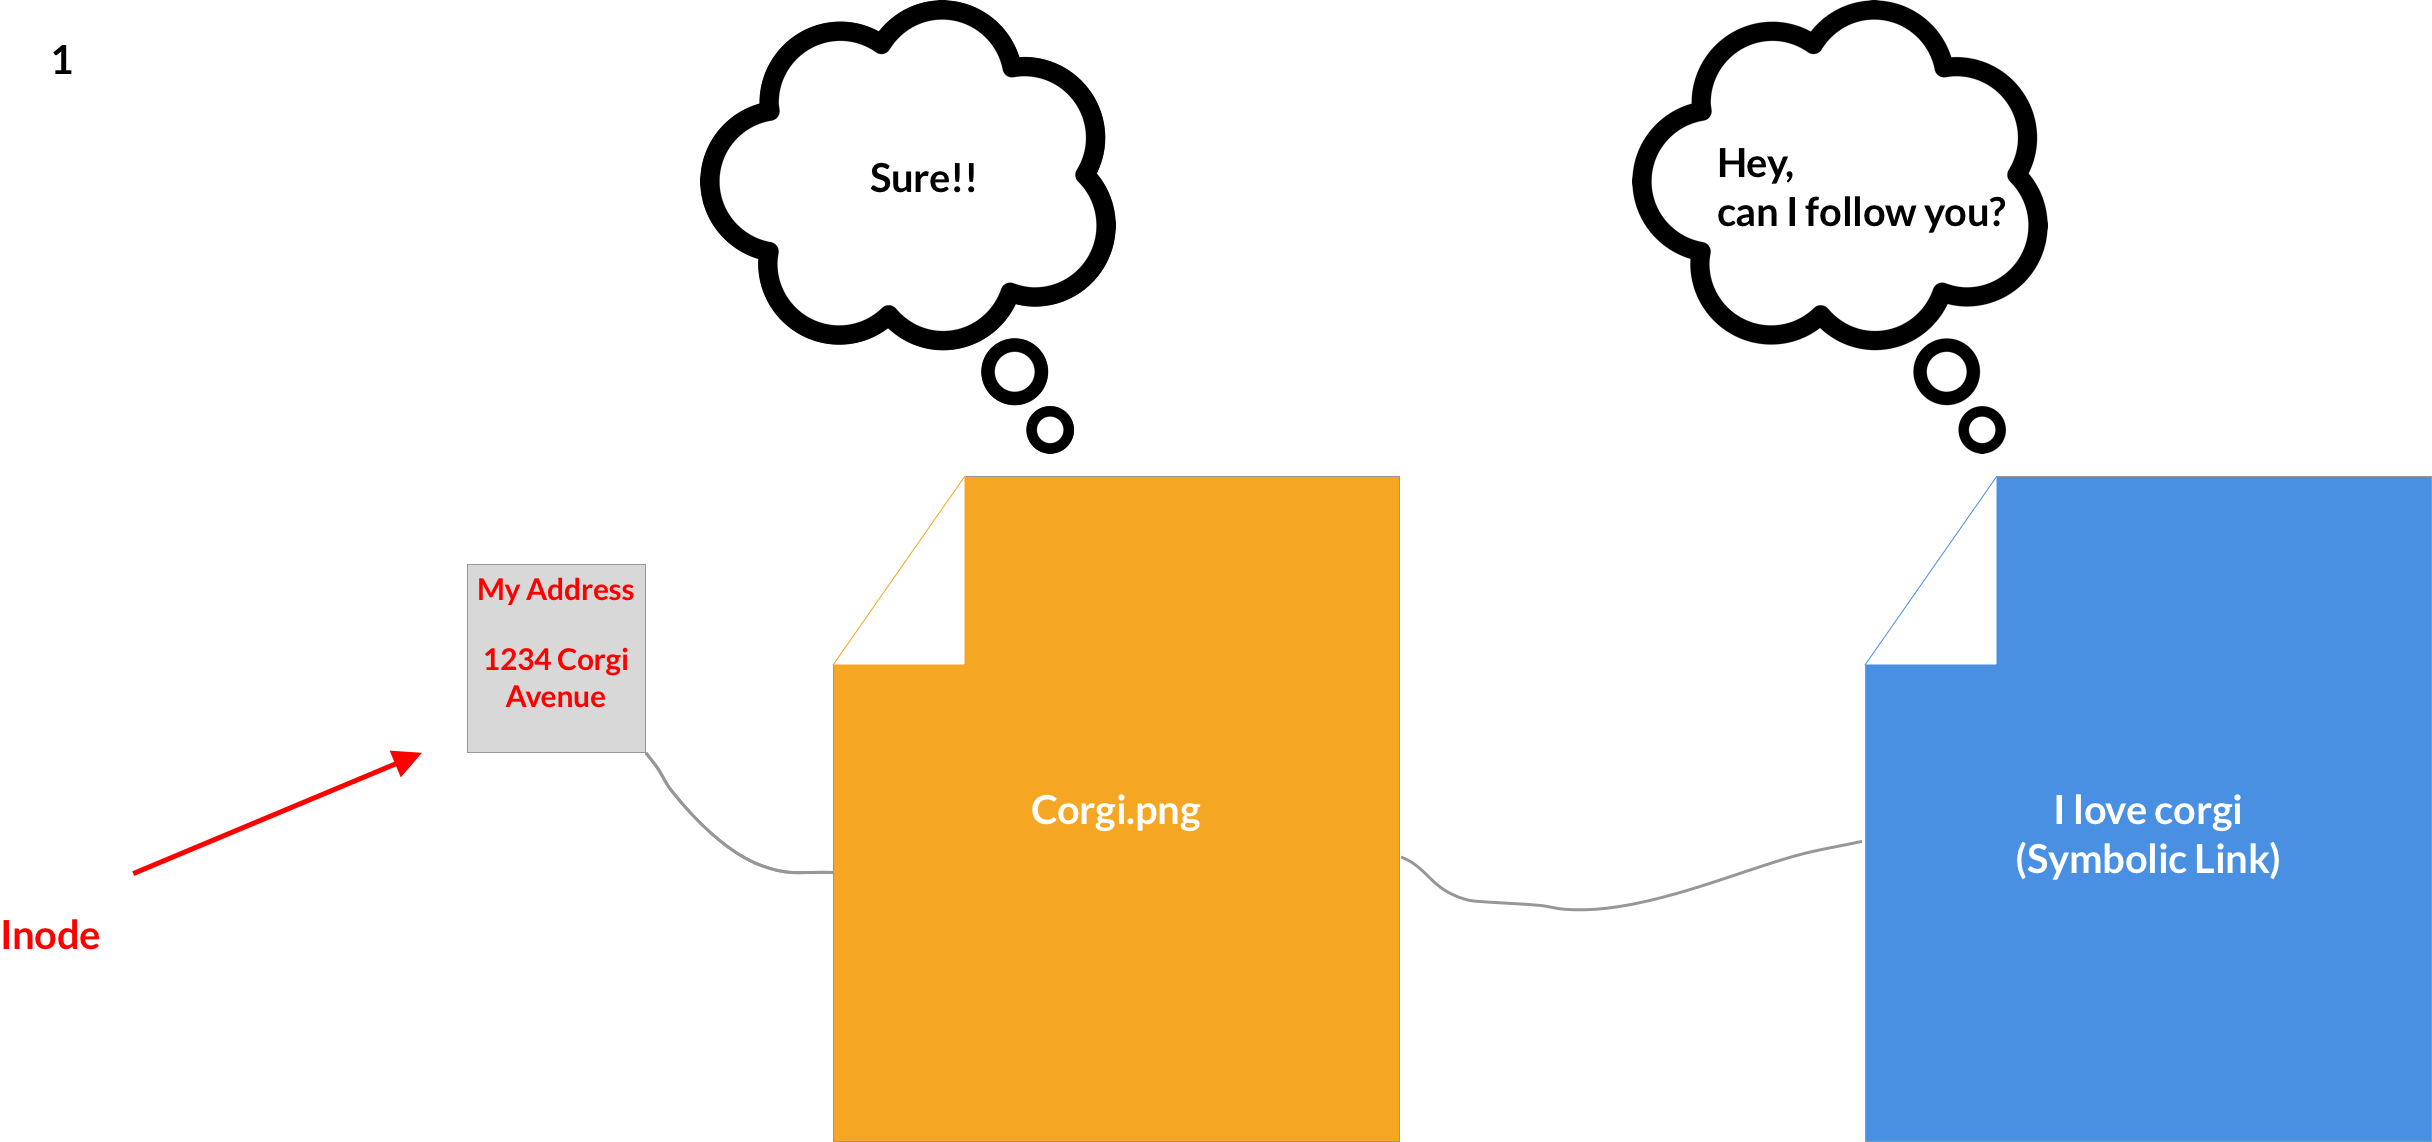
\includegraphics[width=0.8\linewidth]{../images/midterm_4_solution_19.png}
                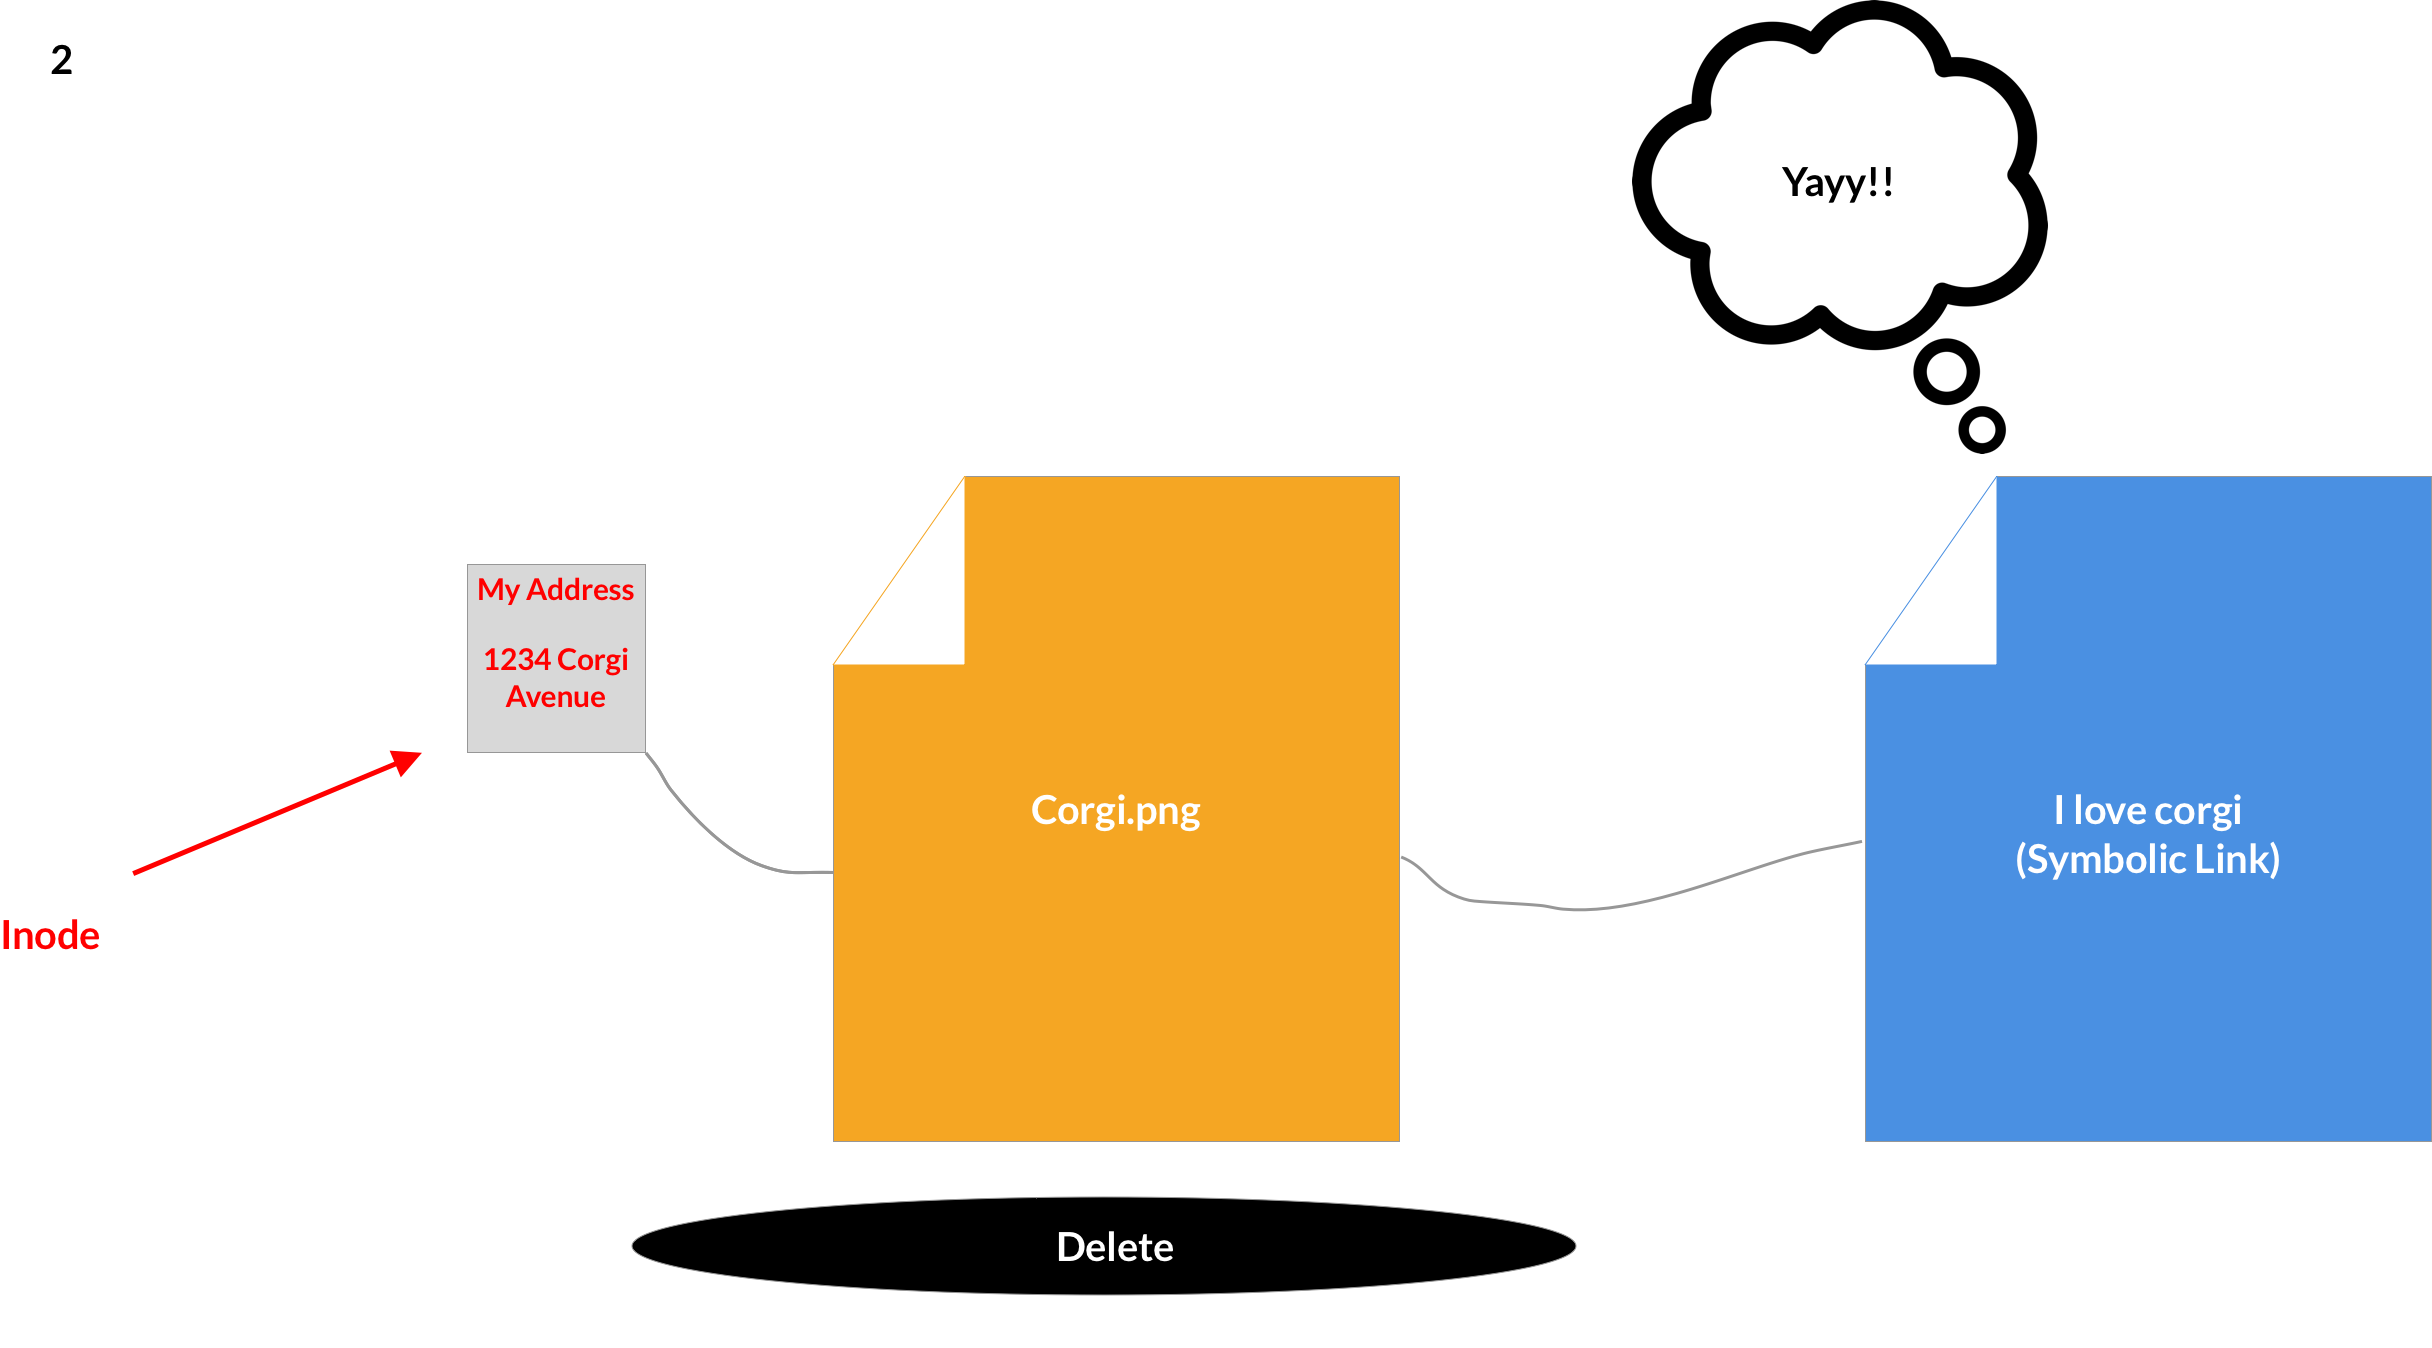
\includegraphics[width=0.8\linewidth]{../images/midterm_4_solution_20.png}
                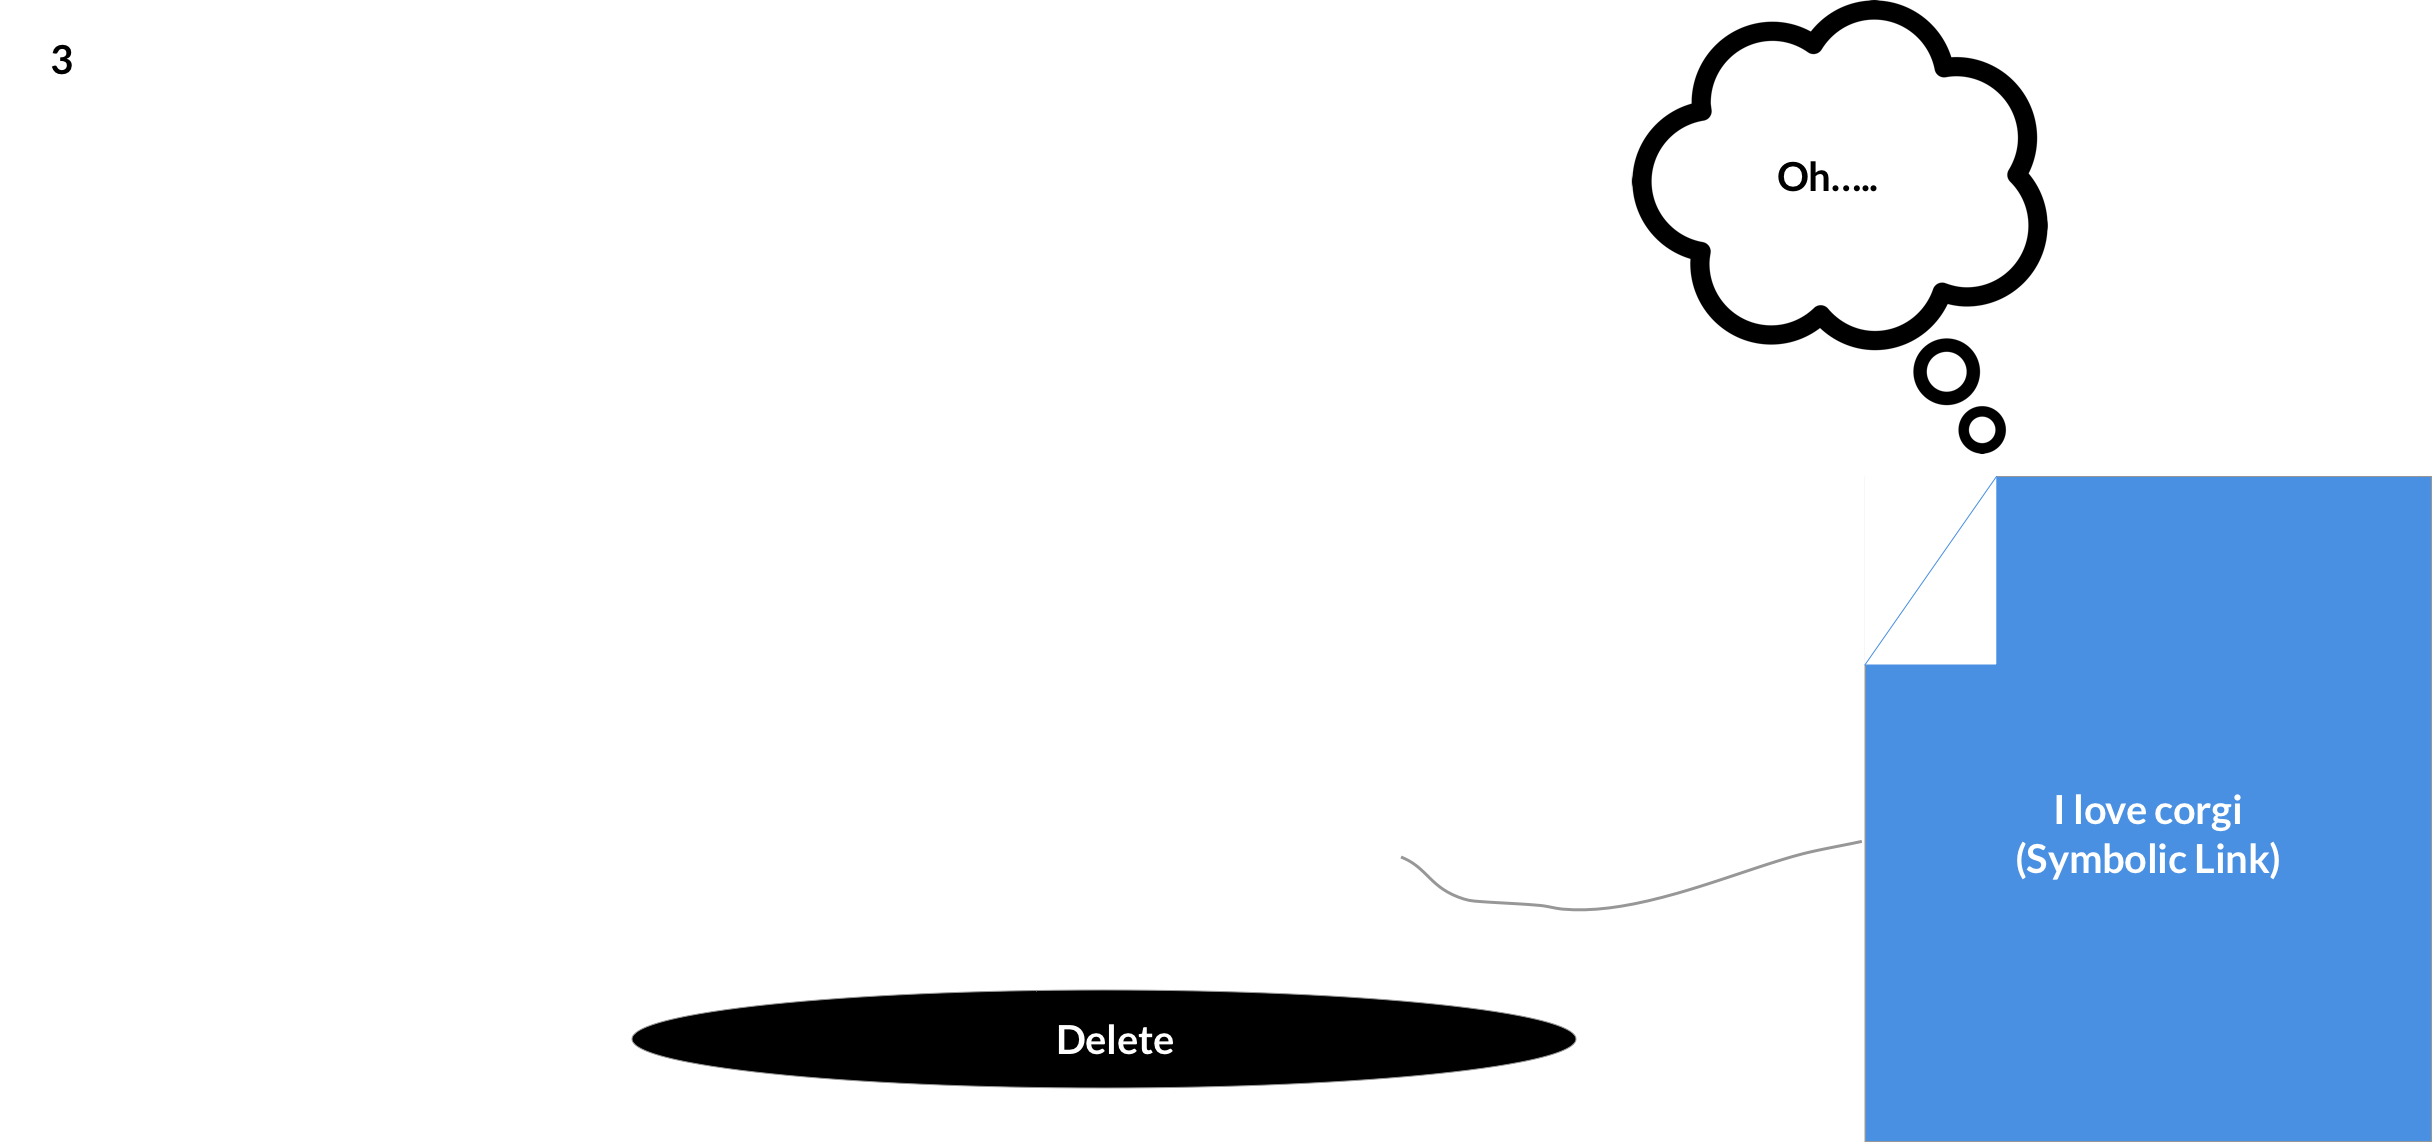
\includegraphics[width=0.8\linewidth]{../images/midterm_4_solution_21.png}
            \end{center}

            \item \textbf{Hard Link:}
            \begin{itemize}
                \item Is a direct reference to a file via its inode $^{[2]}$
                \item Is second directory entry identical to first
            \end{itemize}

            \begin{center}
            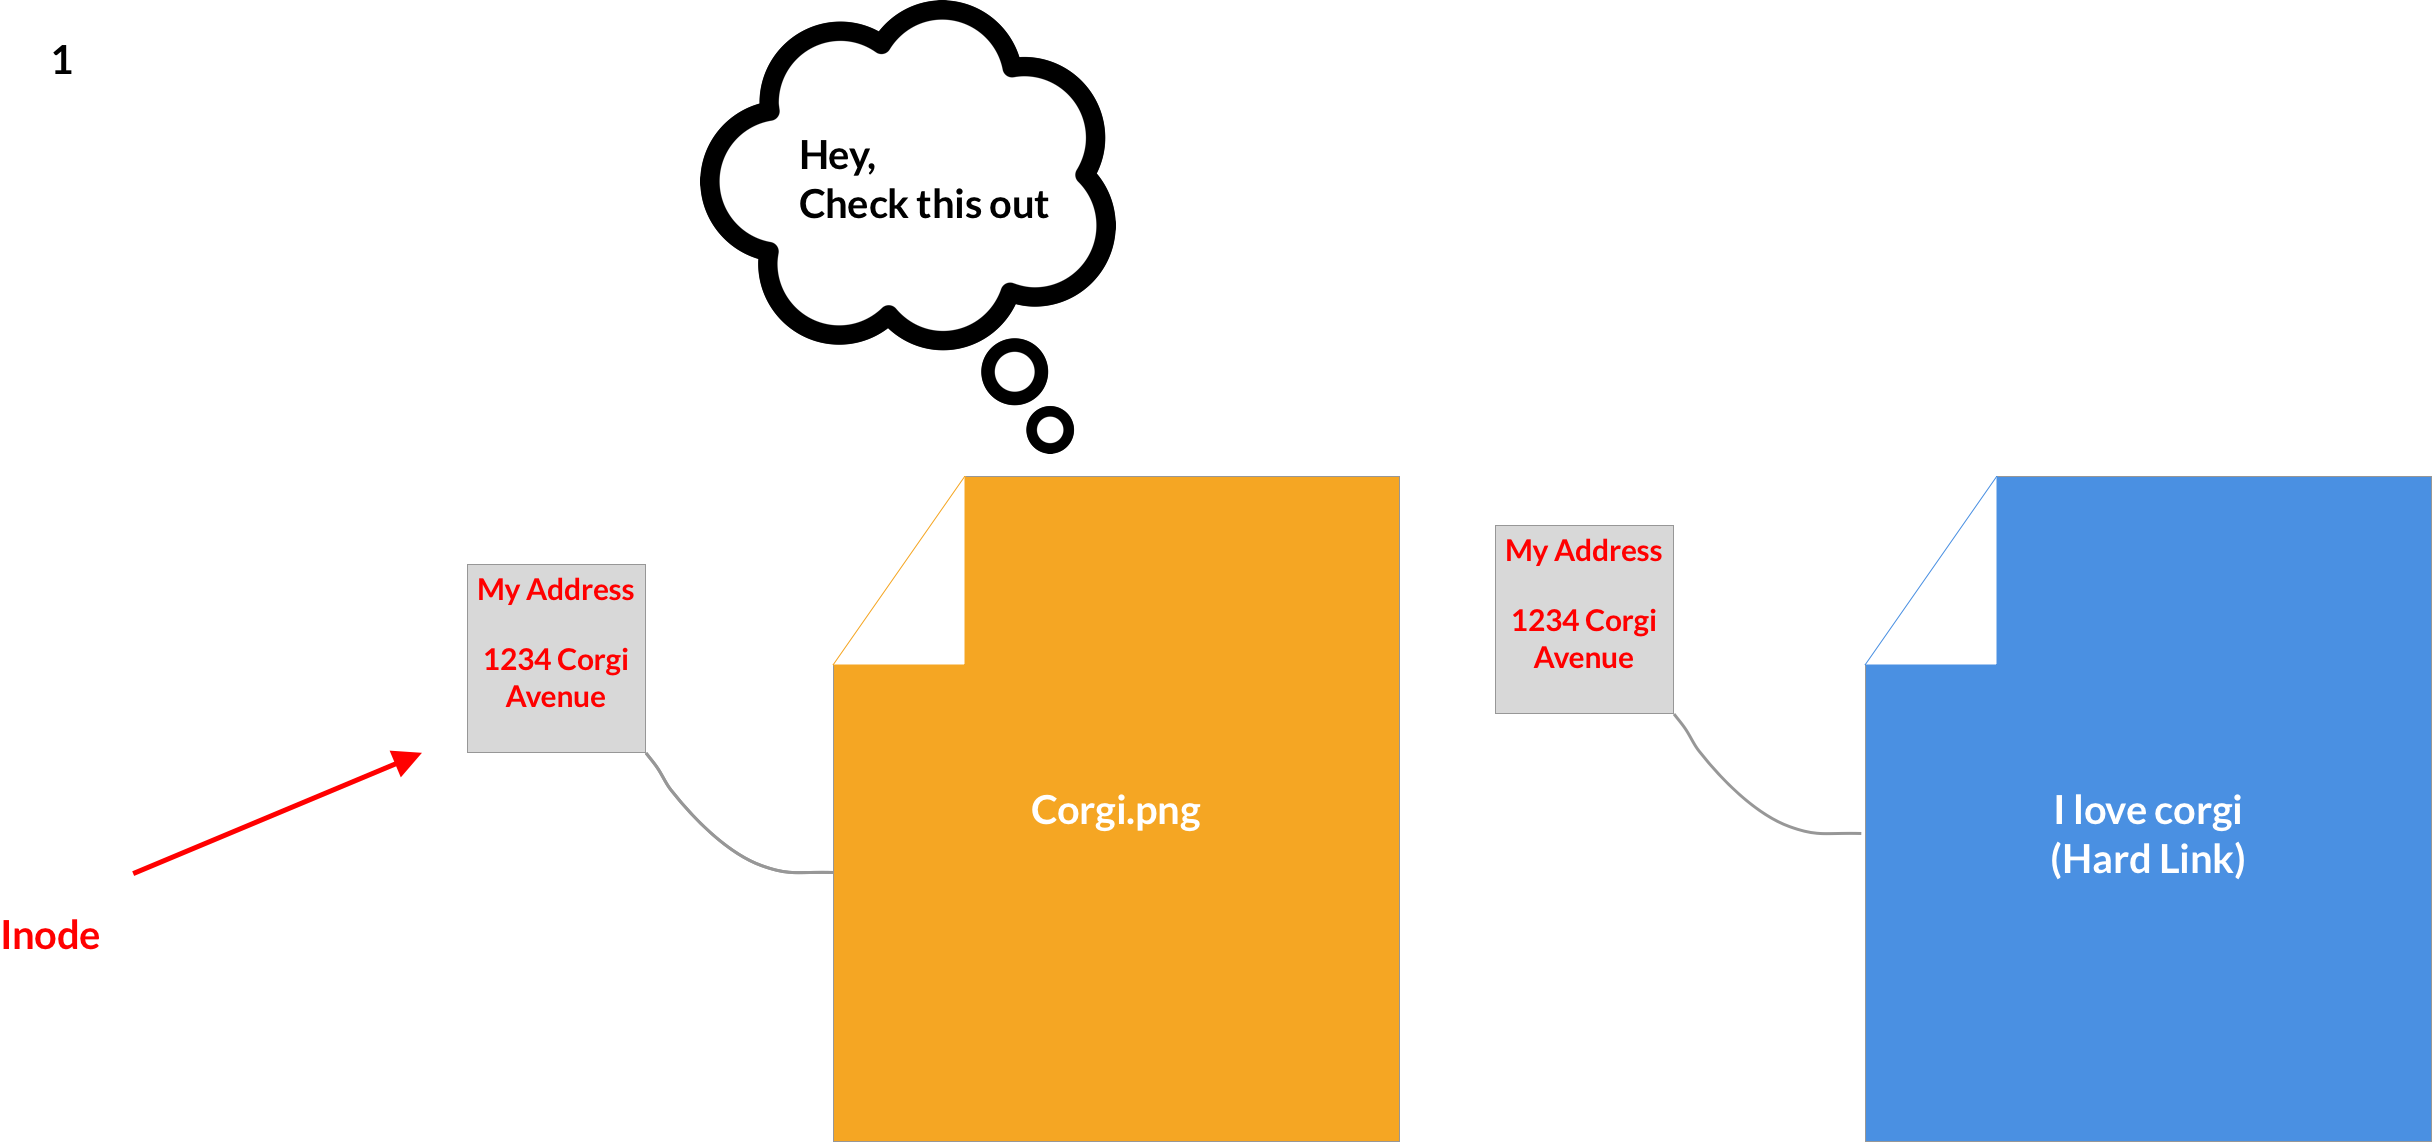
\includegraphics[width=0.8\linewidth]{../images/midterm_4_solution_22.png}
            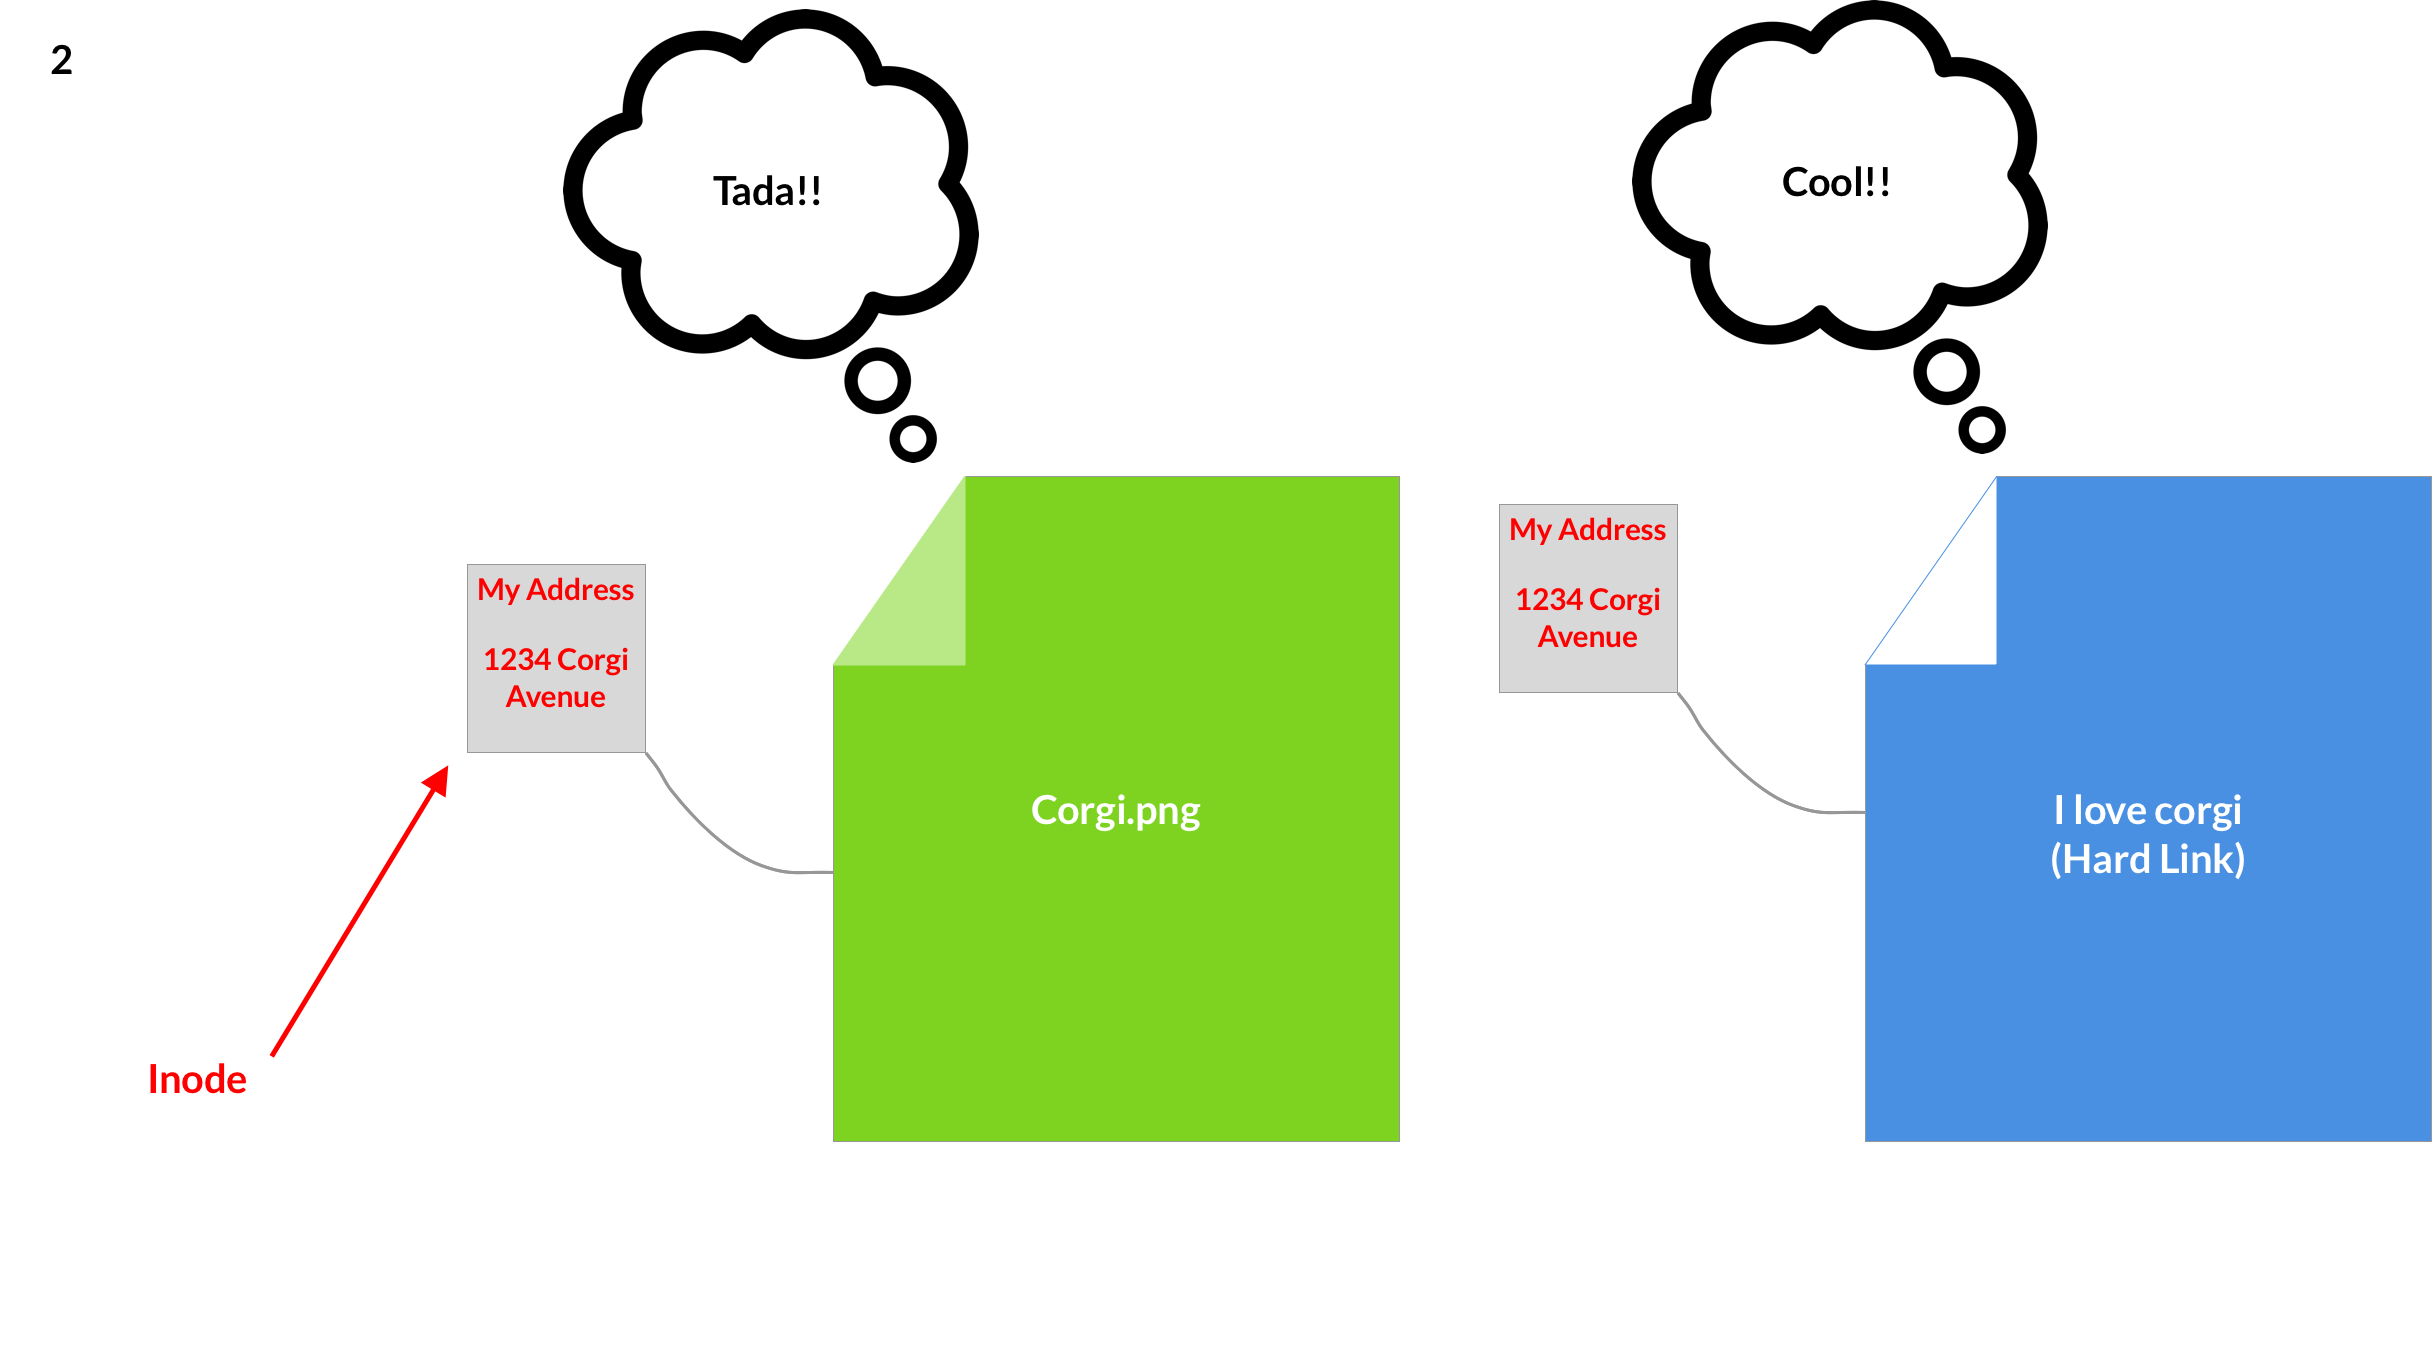
\includegraphics[width=0.8\linewidth]{../images/midterm_4_solution_23.png}
            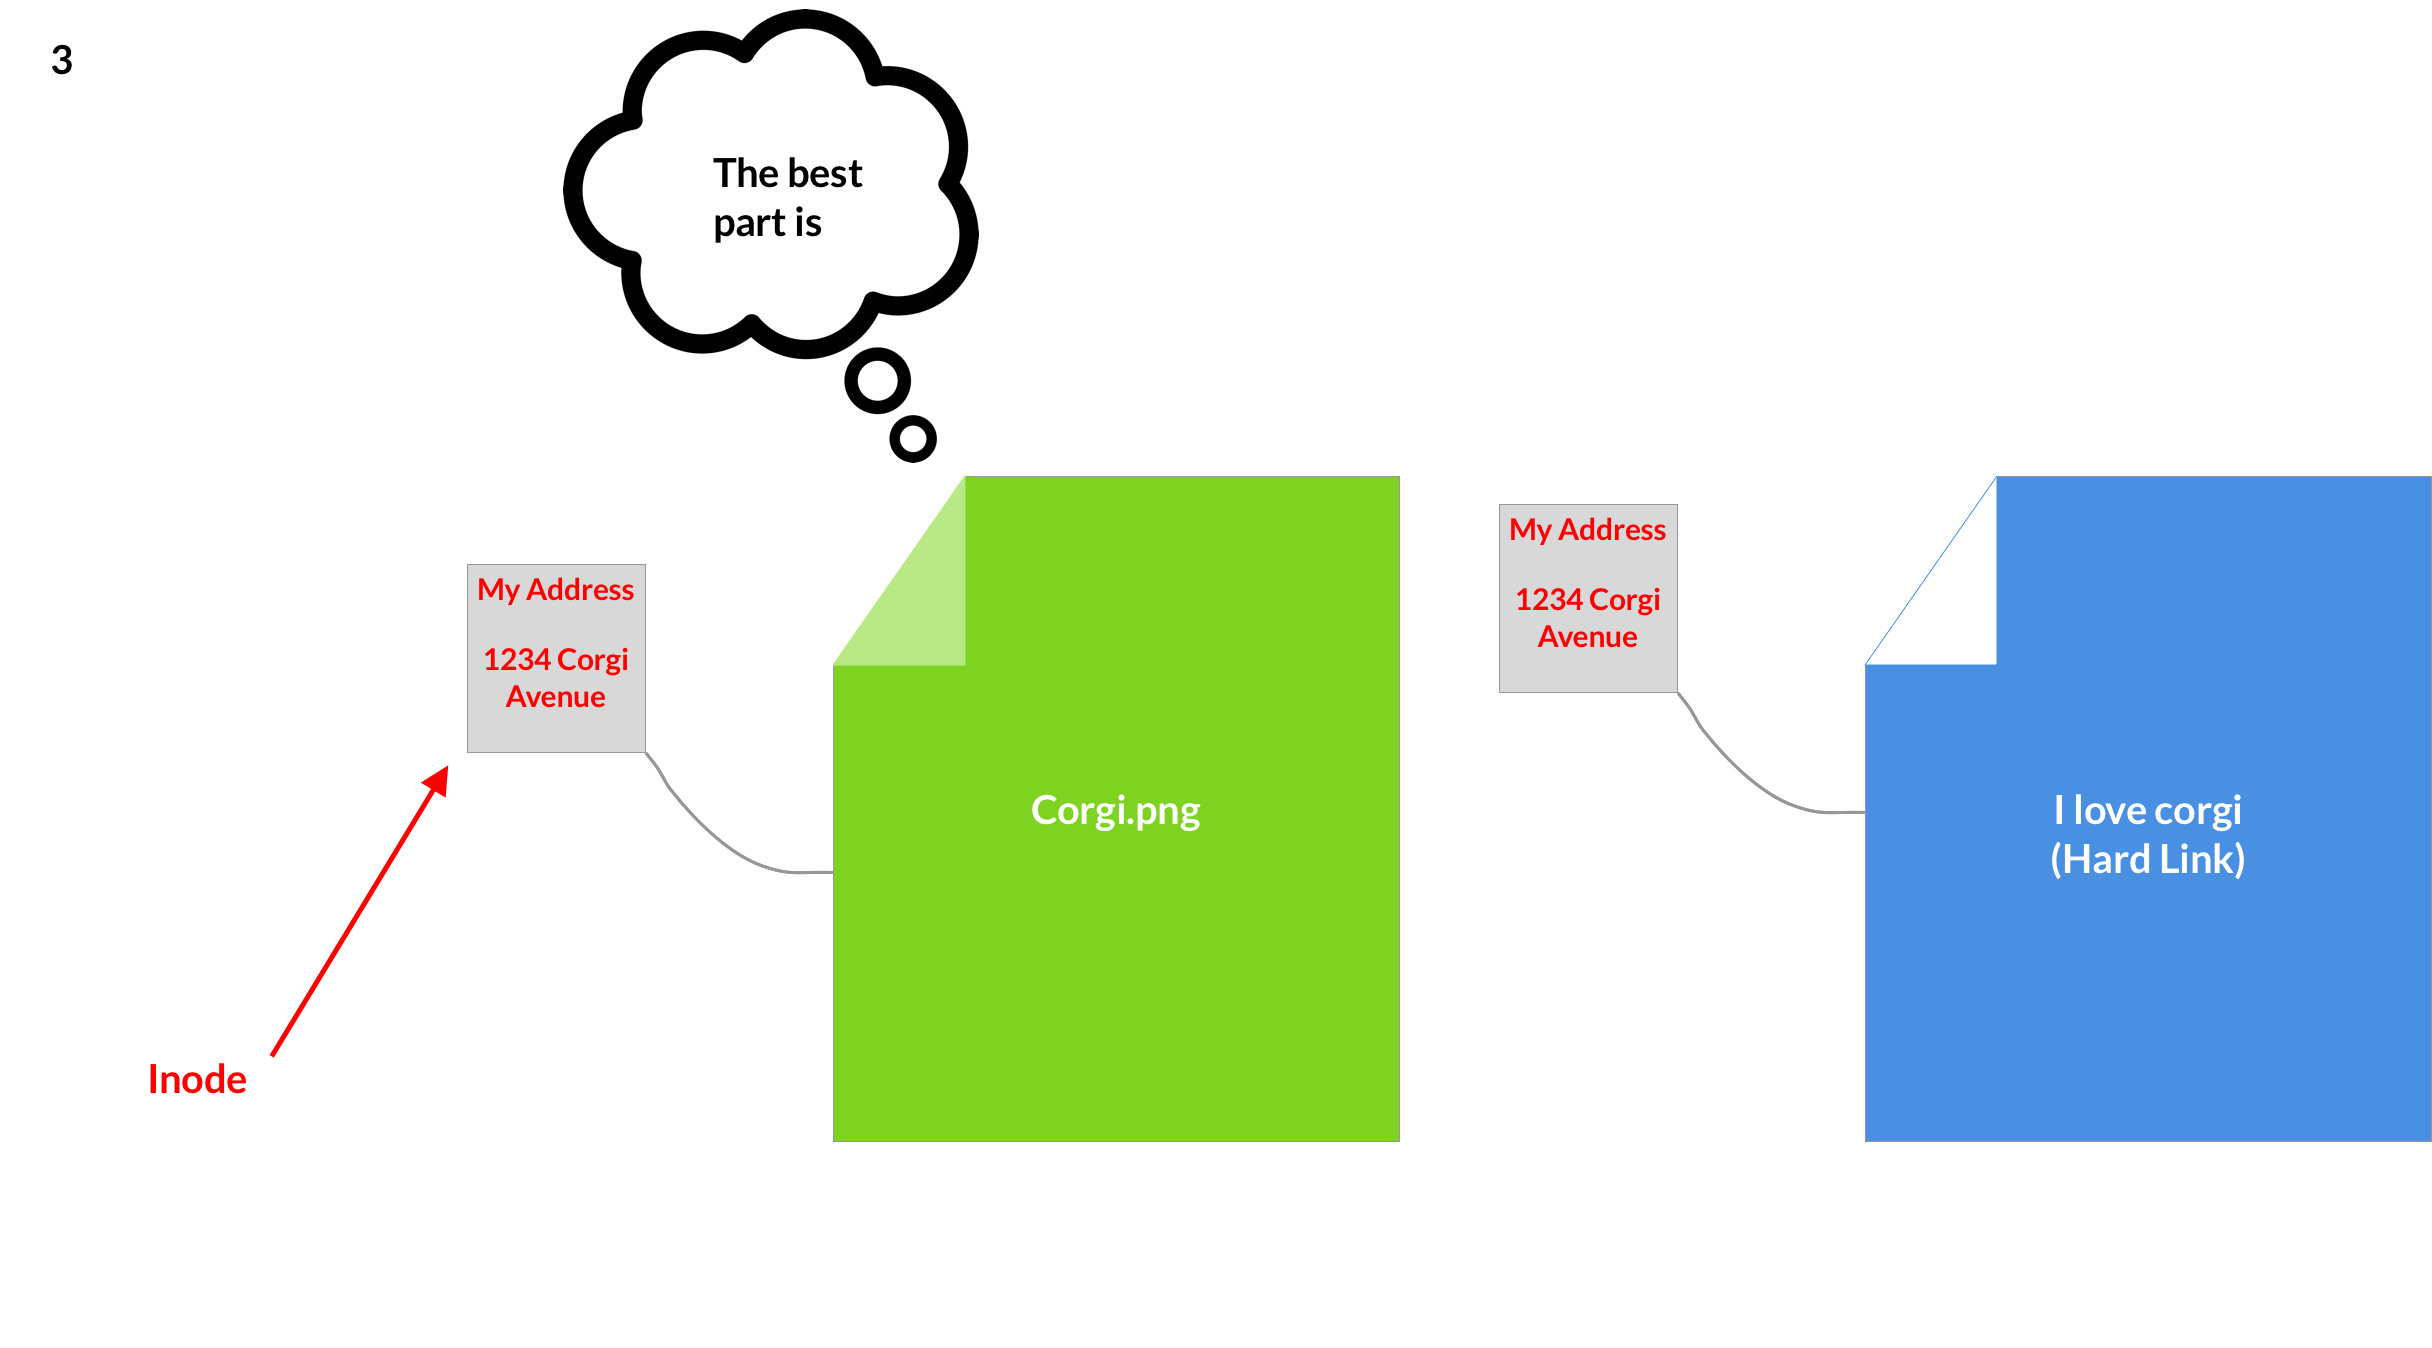
\includegraphics[width=0.8\linewidth]{../images/midterm_4_solution_24.png}
            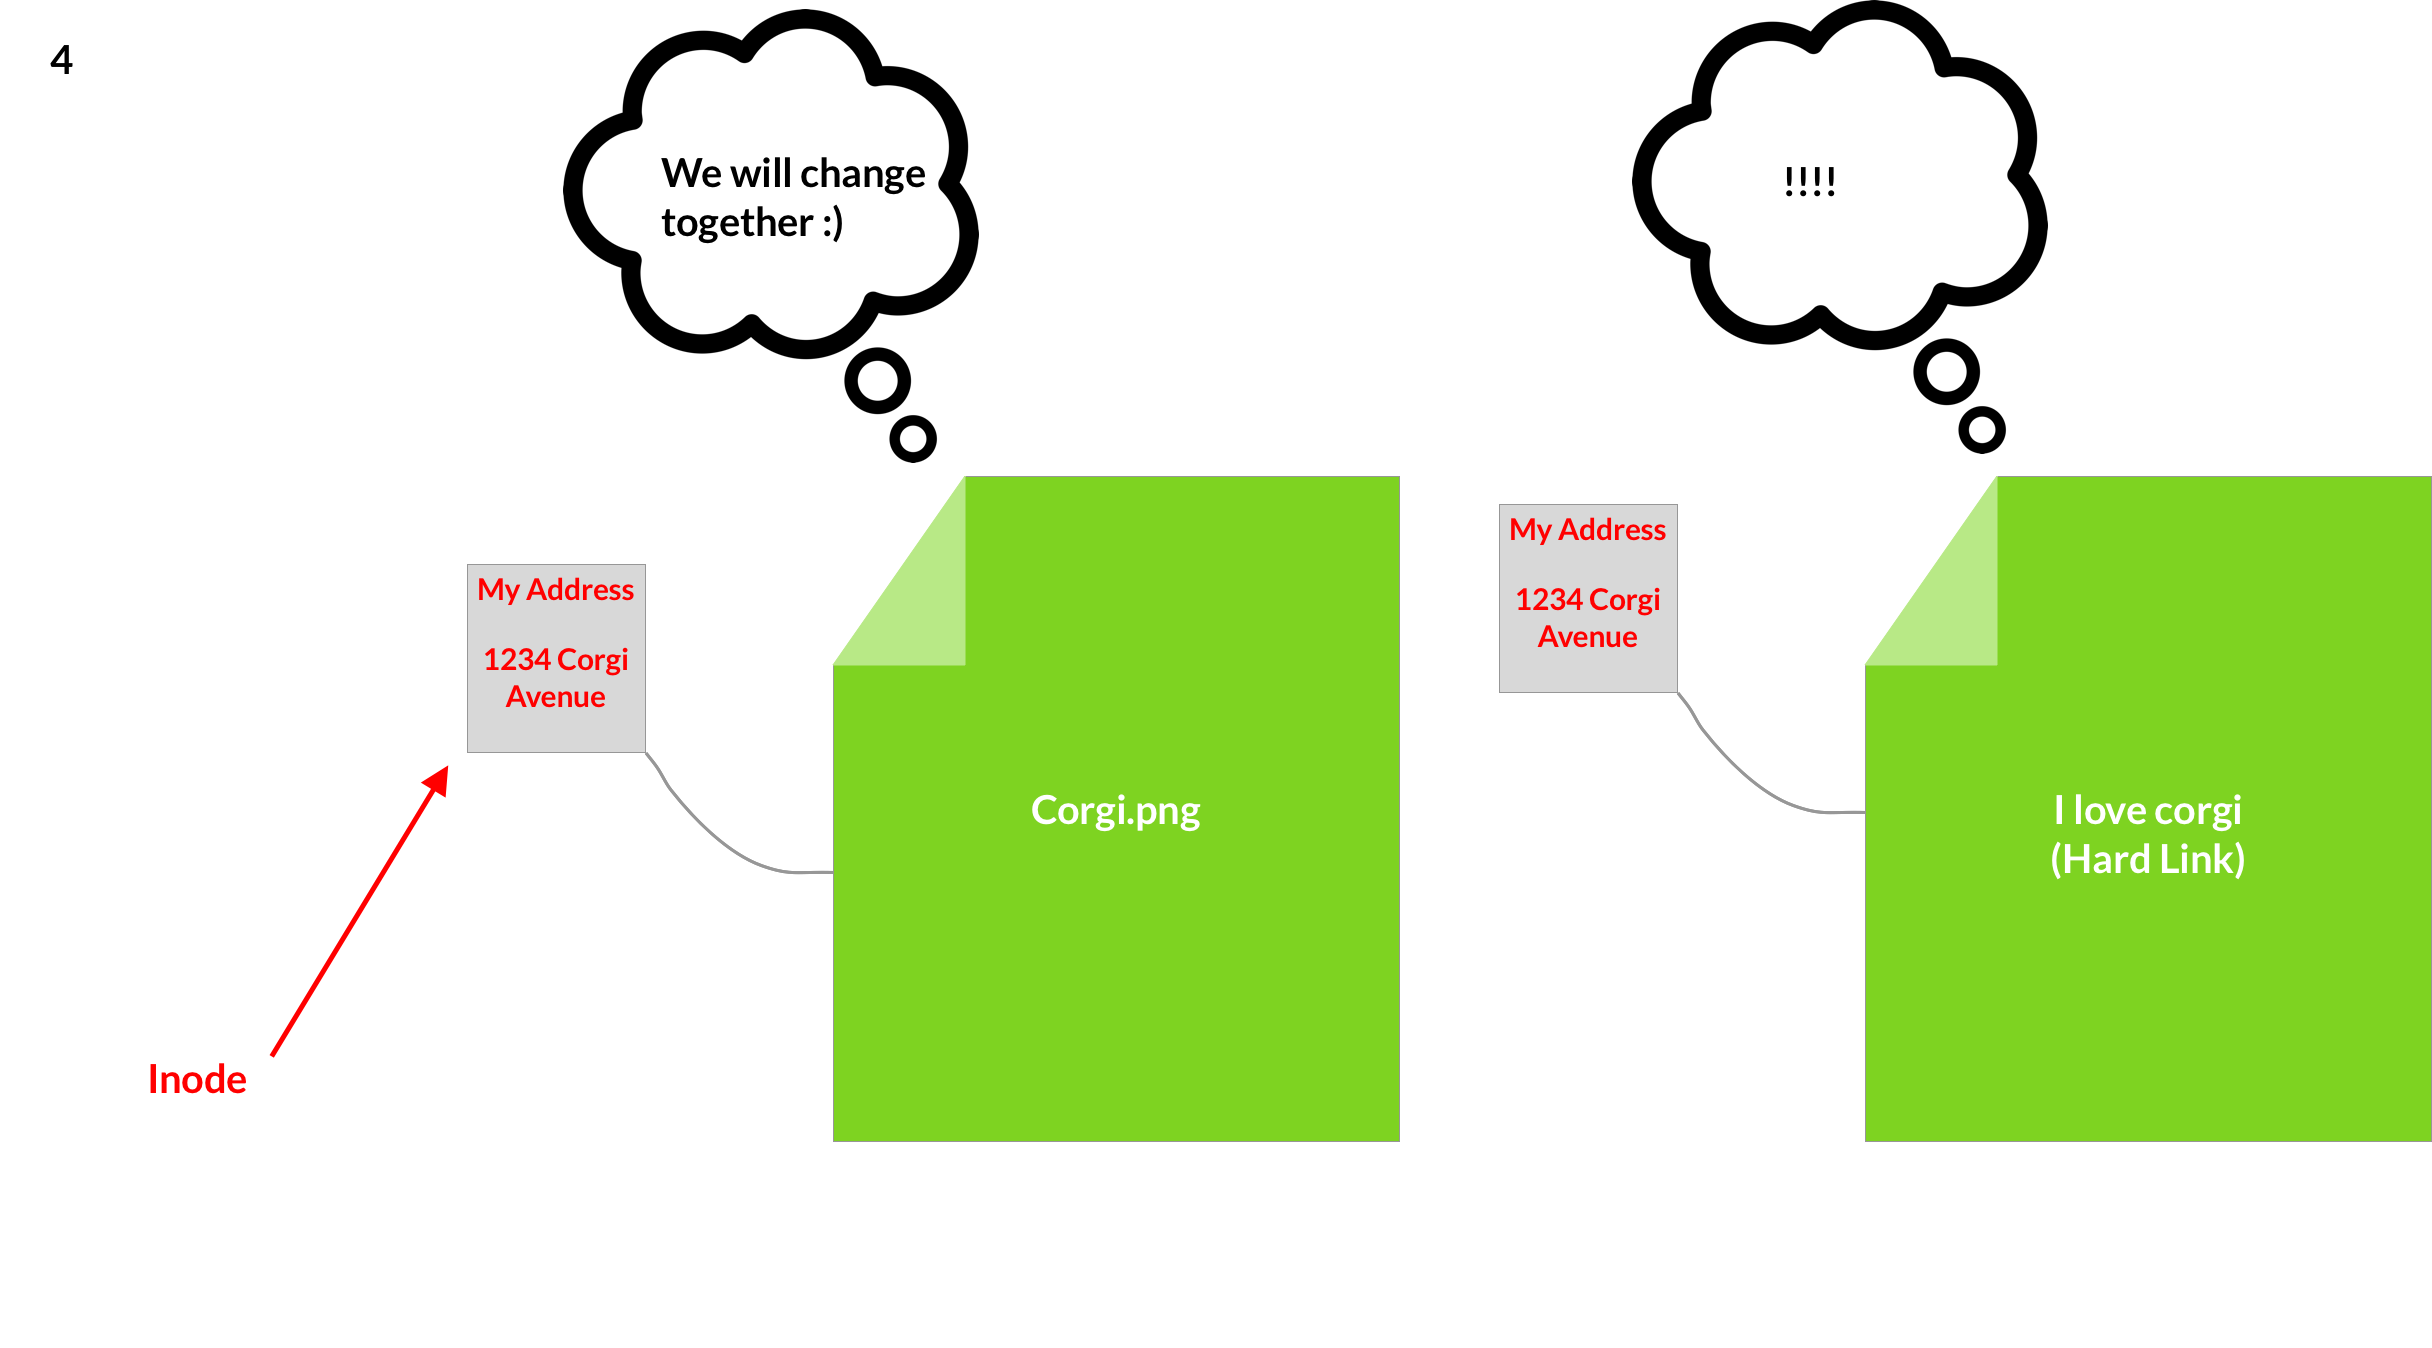
\includegraphics[width=0.8\linewidth]{../images/midterm_4_solution_25.png}
            \end{center}

            \item \textbf{Crash Consistency}

            \begin{itemize}
                \item Inode before update

                \begin{center}
                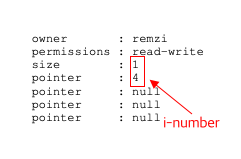
\includegraphics[width=0.6\linewidth]{../images/midterm_4_solution_26.png}
                \end{center}

                \item Inode after update

                \begin{center}
                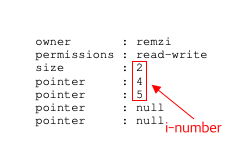
\includegraphics[width=0.6\linewidth]{../images/midterm_4_solution_27.png}
                \end{center}
            \end{itemize}
        \end{itemize}

        \bigskip

        \underline{\textbf{References}}

        \begin{enumerate}[1)]
            \item codewiki, stat, \href{http://codewiki.wikidot.com/c:system-calls:stat}{link}
            \item The Open Group Base Specification, unlink, \href{https://pubs.opengroup.org/onlinepubs/009695399/functions/unlink.html}{link}
        \end{enumerate}
    \end{enumerate}

    \item

    \begin{enumerate}[a)]
        \item Indexed-based file system uses inode number and pointers to find data blocks, and
        data blocks can be set and anywhere, so external fragmentation isn't a problem

        \item Extent based file system only requires a pointer to first data block of file,
        and the rest is read by traveling contiguously, and this requires less disk block access
        than index-based file system of which has to go to inode block, indirect pointers and
        data blocks to go to a particular byte in file.
    \end{enumerate}

    \bigskip

    \underline{\textbf{Notes}}

    \begin{itemize}
        \item What is a sector? What is a sector address?
        \item How can I get to specific inode from block (e.g inode \# 32 on block 2)?
        \item I should record differences between linked-list-based FS, Extent-based FS, and indexed FS
        \item \textbf{Index Based File System}

        \begin{center}
        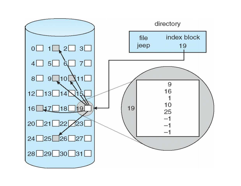
\includegraphics[width=0.6\linewidth]{../images/midterm_4_solution_29.png}
        \end{center}

        \begin{itemize}
            \item Has 15 blocks of pointers that points to either inode, indirect pointers, or data block
            \item No external fragmentation
            \item Files can be easily grown
        \end{itemize}

        \bigskip

        \underline{\textbf{Example}}

        \bigskip

        Linux's ext2, ext3

        \item \textbf{Extent Based File System}

        \begin{center}
        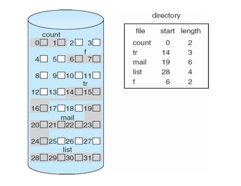
\includegraphics[width=0.7\linewidth]{../images/midterm_4_solution_28.png}
        \end{center}

        \begin{itemize}
            \item Requires only a disk pointer + length (in blocks)
            \item Is also called \textbf{contiguous allocation}
            \item Is simple
            \item Is less flexible but more compact
            \item Works well when there is enough free space on the disk and files can be laid out contiguously

            \bigskip

            \underline{\textbf{Example}}

            \bigskip

            Linux's ext 4
        \end{itemize}
        \item \textbf{inode}
        \begin{itemize}
            \item Inode block computation

            \begin{align}
            \texttt{block number} = (\texttt{inode \#} * \texttt{sizeof(inode)}) / \texttt{block size}
            \end{align}

            \bigskip

            \underline{\textbf{Example}}

            \bigskip

            Target: inode \#32

            Inode Size: 256 bytes

            Block Size: 4096 bytes

            \bigskip

            \begin{align}
            \texttt{block number} &= (\texttt{inode \#} * \texttt{sizeof(inode)}) / \texttt{block size}\\
            &= \frac{32 * 256}{4096}\\
            &= 2
            \end{align}


        \end{itemize}
        \item \textbf{superblock}
        \begin{itemize}
            \item Contains information about the following
            \begin{itemize}
                \item The number of inodes and data blocks in a particular file system
                \item The magic number of some knd to identify the file system type
                \item Where the inode table begins
            \end{itemize}
            \item Is read first on mount before attaching to file system
        \end{itemize}
        \item \textbf{inode/data bitmap}
        \begin{itemize}
            \item Accessed only when allocation/deallocation is needed
            \begin{itemize}
                \item \texttt{Read()} $\to$ no bitmap required
            \end{itemize}
            \item Uses bit to indicate whether the corres object/block is free
            \begin{itemize}
                \item 0 means free
                \item 1 means in use
            \end{itemize}
        \end{itemize}

        \item \textbf{Reading a File from Disk}

        \underline{\textbf{Example}}

        \bigskip

        When

        \bigskip

        \texttt{open("/foo/bar", O\_READONLY)}

        \bigskip

        is called

        \bigskip

        \begin{itemize}
            \item the goal is to find the inode of the file \texttt{bar} to read its basic information
            (i.e. includes permission, information, file size etc)
            \item done by traversing the pathname and locate the desired inode
            \item Steps

            \begin{enumerate}[1.]
                \item Find \textbf{inode} of the root directory by looking for \textbf{i-number} (or
                \textbf{inode number})
                \begin{itemize}
                    \item Root directory has no parent directory
                    \item Root directory's \textbf{inode number} is 2 (for UNIX file systems)
                \end{itemize}

                \item Read the \textbf{inode} of root directory
                \item Once its \textbf{inode} is read, read through its directory data (pointers to \textbf{data blocks})
                until the inode number of \texttt{foo} is found (e.g 42)
                \item Recursively traverse the pathname until the desired inode is found (more specifically, the \textbf{inode number} of bar)
                \item Issue a \texttt{open()} to read \texttt{bar}'s inode to memory
                \item Issue a \texttt{read()} system call to read from file \texttt{bar}

                \begin{itemize}
                    \item without \texttt{lseek()}, reads file from the first file data block (e.g. \texttt{bar data[0]})
                    \item \texttt{lseek(..., offset\_amt * size\_of\_file\_block)} is used to offset/move to desired block in \texttt{bar}
                \end{itemize}

                \item Trasnfer data to \texttt{buf} data block

                \item Read until \texttt{read()} returns 0, or desired data block has been read
                \item Close \texttt{fd}. No I/O is read.
            \end{enumerate}
        \end{itemize}

        \item \textbf{Writing to Disk}

        \begin{center}
        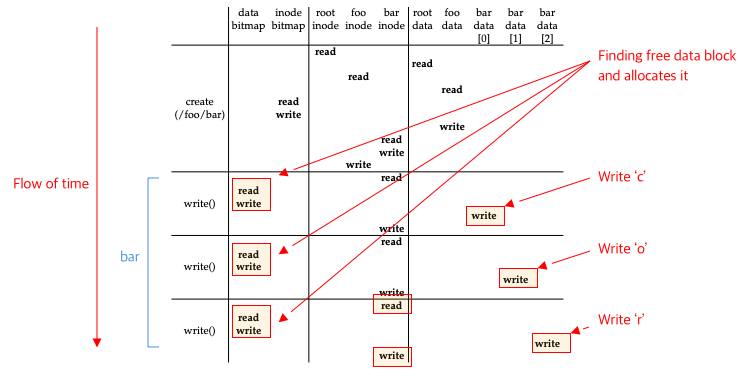
\includegraphics[width=\linewidth]{../images/midterm_4_solution_30.png}
        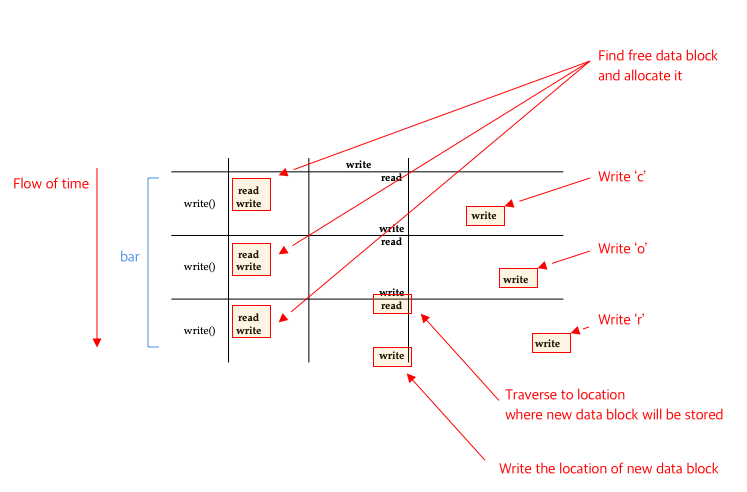
\includegraphics[width=\linewidth]{../images/midterm_4_solution_31.png}
        \end{center}

        \bigskip

        Given a call

        \bigskip

        \texttt{create(...)} (Note: \texttt{open} to be exact)

        \bigskip

        \begin{itemize}
            \item 5 I/Os are generated per write

            \begin{itemize}
                \item Read inode (to traverse to the location of new data block)
                \item Reading data bitmap
                \item Writing data bitmap
                \item Write data block
                \item Write inode (to update data block's location in inode)
            \end{itemize}
            \item 10 I/Os are generated per file creation:

            \begin{itemize}
                \item Read inode bitmap (to find free inode)
                \item Write inode bitmap (to mark it allocated)
                \item Create one new inode (to initialize it)
                \item Write the location of new inode block in \texttt{foo} (by linking high-level name of file \texttt{bar} to its inode number and storing in data block)
                \item Perform one read and write to the directory inode and update it
            \end{itemize}
        \end{itemize}

        \item \textbf{Static Partitioning}

        \begin{itemize}
            \item Divides resources into fixed proportion \underline{once}
            \begin{itemize}
                \item e.g. two possible users of memory $\to$ give fraction of memory to one user and
                rest to the other
            \end{itemize}
            \item Advantages
            \begin{itemize}
                \item Ensures each user receives some share of the resource
                \item Delivers more predictable performance (usually)
                \item Easier to implement
            \end{itemize}
            \item Disadvantages
            \begin{itemize}
                \item Is wasteful
                \item
            \end{itemize}
        \end{itemize}

        \item \textbf{Dynamic Partitioning}

        \begin{itemize}
            \item Gives out different amounts of resources over time
            \item Lets resource-hungry users consume idle resources
            \item Advantages
            \begin{itemize}
                \item Flexible
                \item Can achieve better utilization than \textbf{static partitioning}
            \end{itemize}
            \item Disadvantages
            \begin{itemize}
                \item More complex to implement
                \item Could lead to worse performance
                \begin{itemize}
                    \item e.g idle resource got consumed by others and take long
                    time to reclaim it when needed (the perodic frozen feeling when loading screen)
                \end{itemize}
            \end{itemize}
        \end{itemize}

    \end{itemize}

    \bigskip

    \underline{\textbf{References}}

    \begin{enumerate}[1)]
        \item Columbia University, Operating Systems, \href{https://www.cs.columbia.edu/~junfeng/10sp-w4118/lectures/l25-fs.pdf}{link}
    \end{enumerate}

    \item

    \bigskip

    \begin{enumerate}[1)]
        \item

        \begin{enumerate}[i)]
            \item all of the above
            \item

            To minimize damage, it should be updated in the order of

            \bigskip

            \begin{enumerate}[1.]
                \item Data Region
                \item Inode Table
                \item Data Bitmap
                \item Inode Bitmap
            \end{enumerate}

            \bigskip

            The reason is that when data block and/or inode block are set and
            crash happens, the file system treats as if nothing had happened.

            \bigskip

            And the reason is that before data/inode block is allocated, it first checks
            the inode and data bitmap, which contains information about whether the block is occupied or not.

            \bigskip

            Once they are allocated, we risk data/inode leak, and if done improperly,
            the data/inode block would not be available until actions are taken.
        \end{enumerate}

        \item

        \begin{enumerate}[i)]
            \item inode bitmap, data bitmap
            \item

            To minimize damage, it should be updated in the order of

            \bigskip

            \begin{enumerate}[1.]
                \item Data Bitmap
                \item Inode Bitmap
            \end{enumerate}

            \bigskip

            The reason is that when data bitmap is removed and crash happens,
            The data are still in place, and those can be used to continue the operation
            (assuming that nothing is disturbed).

            \bigskip

            More specifically, deletion of file is complete when reference count in the inode of
            file B hits 0, and as long as data is in place we can work so that the inode's
            reference count hits 0, and the file is removed.

            \bigskip

            However, if done the opposite and crash occurs, we can't remove its data bitmaps,
            and data leak would result.

            \bigskip

            \underline{\textbf{Notes}}

            \begin{itemize}
                \item I really need to know what happens
            \end{itemize}
        \end{enumerate}

        \item

        The primary motiviations behind log-structured file system are as follows

        \begin{enumerate}[1.]
            \item Decrease a large number of intermediary processes during a write in FFS (e.g creation of data block, inode)
            \item Utilize the ever increasing capacity of memory, and write a large block of information at once (to boost performance)
            \item To compensate for the slow development of cheap and fast motor for ever increasing capacity and the need for higher data transfer rate
        \end{enumerate}

        \bigskip

        The update process for log-structured file system works by storing write information
        to in-memory space called \textbf{segment}, and write all once once its at capacity.

        \bigskip

        On the other hand, the writing process of FFS works by traveling to target directory,
        create a inode bitmap, create file inode, update the currect directory inode, create
        a data block in directory inode that points to the file inode, allocate data inode,
        and write data block for file, and update the current file meta data.

        \bigskip

        And this data block writing process continues until all are filled.

        \bigskip

        \underline{\textbf{Notes}}

        \begin{itemize}
            \item \textbf{Log Structured File System}

            \begin{itemize}
                \item Wait. This sounds very similar to \textbf{extent-based file system}
                \item Buffers all updates (including metadata) in an in-memory \textbf{segment},
                and when segment is full, it is written to disk in one long, sequential
                transfer to unused part of the disk
                \item Instead of overwriting files, always writes unused
                portion of the disk, and reclaim the old space through cleaning

                \item Motivations
                \begin{enumerate}[1.]
                    \item \textbf{System memories are growing}
                    \begin{itemize}
                        \item Data is cached in memory
                        \item Reads are serviced by cache
                        \item Disk traffic is increasingly consists of writes
                        \item File performance $\approx$ write performance
                    \end{itemize}
                    \item \textbf{There is a large gap between random I/O performance and
                    sequential I/O performance}
                    \begin{itemize}
                        \item More bits stored on hard drive $\Rightarrow$ bandwith of acessing bits $\uparrow$
                        \item Harder to create cheap, small motors that spin platters faster, and move arm more quickly
                    \end{itemize}
                    \item \textbf{Existing file systems perform poorly on many common workloads}
                    \begin{itemize}
                        \item Many intermediary writes performed per data block (e.g. Bitmap, inode, data block)
                        \item Many short seeks + rotation delays = performance less than the peak
                    \end{itemize}
                    \item \textbf{File systems are not raid aware}
                \end{enumerate}

                \item How it works (Writing to Disk)

                \bigskip

                Basic idea: Write all updates (e.g. data blocks inodes) to the
                disk sequentially (\textbf{write buffering})

                \bigskip

                \begin{enumerate}[1.]
                    \item Buffer updates in an in-memory \textbf{segment}
                    \item Write the \textbf{segment} all at once sequentially when received sufficient number of updates
                \end{enumerate}

                \item Advatages

                \begin{enumerate}[1.]
                    \item Has very high performance
                \end{enumerate}

                \item Disadvantages

                \begin{enumerate}[1.]
                    \item Is complex
                    \item Generates lots of garbages
                    \item Scattered old data. Needs to run \textbf{compaction} periodically $^{[2]}$
                \end{enumerate}
            \end{itemize}

            \item \textbf{Fast File System}
            \begin{itemize}
                \item Divides inode tables into chunks and stores in different cylinder groups
                \item Advantages
                \begin{itemize}
                    \item No external fragmentation
                \end{itemize}
                \item Disadvantages
                \begin{itemize}
                    \item Extra overhead: creates and updates many intermediary files (inode, data block) during a write
                \end{itemize}
            \end{itemize}
        \end{itemize}

        \bigskip

        \underline{\textbf{Refernces:}}

        \bigskip

        \begin{enumerate}[1)]
            \item Ousterhout J. (1991). \textit{The Design and Implementation of a Log-Structured File System}. \href{https://people.eecs.berkeley.edu/~brewer/cs262/LFS.pdf}{link}
            \item Cornell University, Log-Structured File Systems, \href{http://www.cs.cornell.edu/courses/cs4410/2015su/lectures/lec20-lfs.html#:~:text=The%20downside%20of%20storing%20the,or%20inode)%20in%20the%20segment.}{link}
        \end{enumerate}

        \item

        \bigskip

        The challenge of locating data and metadata on LFS is that both data block and inodes are
        not at the fixed position.

        \bigskip

        To compensate for this, LFS has imap that contains the pointers to (i.e. address of)
        the inode with the latest information, but imap is also placed along side inode
        and data block.

        \bigskip

        To compensate for this, LFS has checkpoint region at fixed location that contains the pointers to (i.e. address of)
        the imap with the latest information.

        \bigskip

        So when LFS loads, it first reads the checkpoint regions, upload all imap to in-memory, and when file system gives target inode number, it
        finds inode and its data blocks from there much like UNIX file system.

        \bigskip

        \underline{\textbf{Notes}}

        \begin{itemize}
            \item \textbf{Log Structured File System (cont')}
            \begin{itemize}
                \item Data Block
                \begin{itemize}
                    \item Is found by looking for \textbf{inode} that point to it
                \end{itemize}

                \bigskip

                \begin{center}
                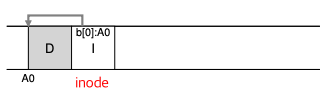
\includegraphics[width=0.8\linewidth]{../images/midterm_4_solution_32.png}
                \end{center}
                \item Inode
                \begin{itemize}
                    \item Stores metadata of file
                    \item Is the same as UNIX file system inode
                    \begin{itemize}
                        \item Has indirect pointers
                        \item Has direct pointers
                        \item Has double indirect pointers
                    \end{itemize}
                    \item Is found through a data structure called \textbf{inode map}
                    \item Are scattered throughout the disk \& keeps moving after update
                \end{itemize}

                \bigskip

                \begin{center}
                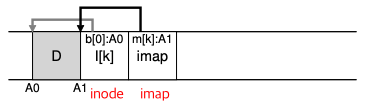
\includegraphics[width=0.8\linewidth]{../images/midterm_4_solution_33.png}
                \end{center}

                \item Inode Map

                \begin{itemize}
                    \item Is a data structure
                    \item Is also moving
                    \begin{itemize}
                        \item new data block, inode and imap are placed contiguously
                    \end{itemize}
                    \item Locates inode
                    \item Takes inode number as input
                    \item Produces the disk address of the most recent version of the inode
                \end{itemize}

                \item Checkpoint Region

                \begin{itemize}
                    \item Is fixed
                    \item Locates imap
                    \item Contains pointers to (i.e. address of) the latest pieces of inode map
                    \item Is updated periodically (e.g every 30 seconds)
                    \begin{itemize}
                        \item Done to ill-affect performance
                    \end{itemize}
                \end{itemize}

                \item How it works (Reading the Disk)

                \begin{enumerate}[1.]
                    \item Read the checkpoint region
                    \item Read the entire inode map and cache it in memory
                    \item Locate inode given inode number of file
                    \item Proceed the same as typical UNIX file system
                \end{enumerate}
            \end{itemize}
        \end{itemize}
    \end{enumerate}

    \item

    \begin{enumerate}[a)]
        \item

        \bigskip

        I am not too sure, but I can deduce as follows:

        \bigskip

        A crash occured while deleting directory \texttt{bart}.

        \bigskip

        \texttt{file1} inode is removed, but due to crash, inode bitmap remained

        \bigskip

        Unless intervened, the block may never be available.

        \bigskip

        \underline{\textbf{Notes}}

        \begin{itemize}
            \item \textbf{Crash Consistency Problem}

            \begin{itemize}
                \item Desired: \textbf{atomic} updates. That is, on crash,
                the file on write is either in (state 1 - before the file got updated)
                or (state 2 - after the file got updated)
                \item Reality: This is not possible
                \item Is the reason why computers have 'Don't turn off computer' message
            \end{itemize}

            \item \textbf{File System Checker}

            \begin{itemize}
                \item Is implemented in early file system
                \begin{itemize}
                    \item Basic Idea: Let inconsistencies happen and fix them later (when rebooting)
                \end{itemize}
                \item Is used by UNIX tool \textbf{fsck} ('file system checker')
                \item Summary of how it works

                \begin{itemize}
                    \item \textbf{Inode State}
                    \begin{itemize}
                        \item Corruption in file is checked (e.g. does it have valid file type such as directory file, or links)
                        \item Solved by removing it, and updating the bitmap if inode cannot be fixed easily
                    \end{itemize}
                    \item \textbf{Inode links}
                    \begin{itemize}
                        \item Number of references in each inode is checked
                        \item Check is done by reading the entire directory tree and building its own link count
                        \item Solved by fixing the count if there is mismatch, or by moving to \texttt{lost+found}
                        directory if there is no directory refers to it
                    \end{itemize}
                    \item \textbf{Duplicates}
                    \begin{itemize}
                        \item Duplicate pointers (i.e. two different inodes pointing to same block) is checked
                        \item Solved by either removing one of two inodes, or creating a copy for each
                    \end{itemize}
                    \item \textbf{Bad Blocks}

                    \begin{itemize}
                        \item A pointer that points to something outside is partition is checked
                        \item Solved by removing the block
                    \end{itemize}

                    \item \textbf{Directory Checks}

                    \begin{itemize}
                        \item Making sure that \texttt{.} and \texttt{..} are first entry is checked
                        \item Allocation of inodes referred to in a directory entry is checked
                        \item Making sure that no directory is linked more than once is checked
                    \end{itemize}
                \end{itemize}

                \item Disadvantage
                \begin{itemize}
                    \item Way too slow. May take Hours.
                    \item Wasteful (Make mistake once, and check everything)
                    \item Doesn't solve all problems (e.g. inode with incorrect data blocks)
                \end{itemize}
            \end{itemize}
        \end{itemize}

        \item

        When online, user would go around, and work on tasks such as downloading music,
        coding, or writing documents using Microsoft Word, it's possible that one of
        the blocks from crash are already in use by others.

        \bigskip

        Because \texttt{fsck} corrects bad blocks, duplicates, inconsistencies in inode metadata, and
        directories, it's possible that on correction, the normal files and directories may become corrupted. (not good)

        \item

        \bigskip

        \underline{\textbf{Notes}}

        \begin{itemize}
            \item After step 4 of data journaling, where are the next transaction begin and end placed?
            \item \textbf{Journaling}
            \begin{itemize}
                \item Is a popular solution to \textbf{crash-consistency problem}
                \item Many file systems use this idea (e.g. ext3, ext4, windows NTFS)
                \item Basic idea

                \begin{itemize}
                    \item before overwriting the structures in place, write down
                    (in a well-known location) a little note of what you are about to do
                    \item If crash occurs, read note and try again
                \end{itemize}

                \bigskip

                \begin{center}
                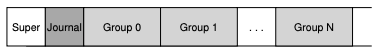
\includegraphics[width=0.8\linewidth]{../images/midterm_4_solution_34.png}
                \end{center}

                \item Advantage

                \begin{itemize}
                    \item Greatly reduces amount of work required during recovery
                \end{itemize}
            \end{itemize}

            \item \textbf{Transaction Beginning (TxB)}
            \begin{itemize}
                \item Where does computer read update instruction (journal ? journal superblock ?)?
                \item In data Journaling, where is comitted data generated and stored prior to putting it in file system?
                \item Includes information about current update
                \item Contains \textbf{Transaction Identifier} or TID
            \end{itemize}

            \item \textbf{Transaction End (TxE)}
            \begin{itemize}
                \item Is marker of the end of transaction
                \item Also contains \textbf{Transaction Identifier} or TID
            \end{itemize}

            \item \textbf{Checkpointing}
            \begin{itemize}
                \item Act of overwriting of old structure in the file system between
                \textbf{transaction beginning} and \textbf{transaction end}
            \end{itemize}

            \item \textbf{Journaling Superblock}

            \begin{itemize}
                \item Records information on which transactions have not yet been checkpointed
                \item Oldest and newest non-checkpointed transactions exist here
                \item Is different from file system superblock
            \end{itemize}
            \item \textbf{Data Journaling}

            \begin{center}
            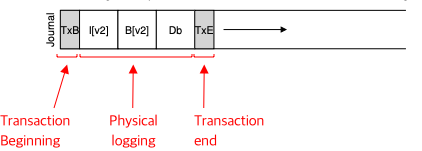
\includegraphics[width=0.8\linewidth]{../images/midterm_4_solution_35.png}
            \end{center}

            \begin{itemize}
                \item Steps

                \begin{enumerate}[1.]
                    \item \textbf{Journal Write}: Write the contents of the transaction (including TxB, metadata and data)
                    to log

                    \begin{center}
                    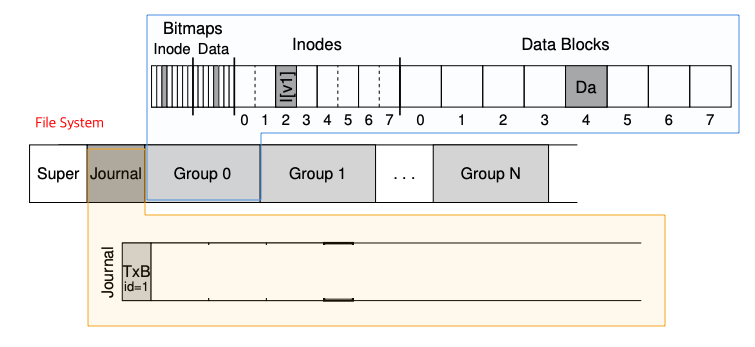
\includegraphics[width=0.8\linewidth]{../images/midterm_4_solution_36.png}
                    \end{center}

                    \item \textbf{Journal Commit:} Write the transaction commit block (containing TxE) to log; wait wait for write to complete

                    \begin{center}
                    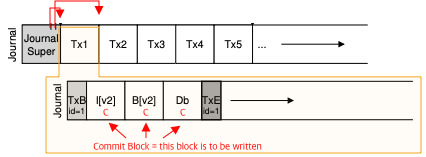
\includegraphics[width=0.8\linewidth]{../images/midterm_4_solution_37.png}
                    \end{center}

                    \item \textbf{Checkpoint:} Write the contents of the update (metadata and data) to their final on-disk location

                    \begin{center}
                    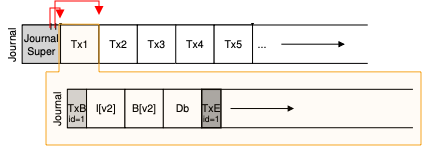
\includegraphics[width=0.8\linewidth]{../images/midterm_4_solution_38.png}
                    \end{center}

                    \item \textbf{Free:} Mark the transaction free in the journal by updating the
                    journal superblock

                    \begin{center}
                    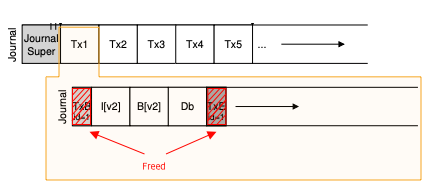
\includegraphics[width=0.8\linewidth]{../images/midterm_4_solution_39.png}
                    \end{center}

                    \item Repeat until done
                \end{enumerate}

                \item Disadvantage

                \begin{itemize}
                    \item Each data block is written twice
                \end{itemize}

                \item Recovery Steps

                \begin{itemize}
                    \item Crash at step 1 $\to$ skip pending update
                    \item Crash during step 2 and 3 $\to$ replay the update

                    \begin{itemize}
                        \item Happens during boot
                    \end{itemize}
                \end{itemize}
            \end{itemize}

            \item \textbf{Metadata Journaling}
            \begin{itemize}
                \item Writes directly to file system without writing to log
                \item Is order dependent
                \item Advantage
                \begin{itemize}
                    \item Solves double write problem in \textbf{data journaling}
                \end{itemize}
                \item Disadvantage
                \begin{itemize}
                    \item
                \end{itemize}
            \end{itemize}
        \end{itemize}

    \end{enumerate}

\end{enumerate}


\end{document}